\documentclass[twoside,10pt]{article}

\usepackage[margin=1in]{geometry} 
\usepackage{amsthm}
\usepackage{amssymb}
\usepackage{amsfonts}
\usepackage[framemethod=TiKZ]{mdframed} 
\usepackage{xcolor}
\usepackage{mathtools}
\usepackage{enumerate}
\usepackage{cancel}

\usepackage{polski}
\usepackage{wasysym}
\usepackage[utf8]{inputenc}

\usepackage{tikz}
\usetikzlibrary{calc,angles,quotes}

\usepackage[symbol]{footmisc}
\usepackage{fancyhdr}
%\setlength{\headheight}{15.2pt}

\pagestyle{fancy}
\fancyhf{}
\fancyhf[ELH,ORH]{\thepage}
\fancyhead[C]{Topologia}

\baselineskip=1.6\baselineskip

\definecolor{lightgray}{gray}{0.96}

\renewcommand{\thefootnote}{\fnsymbol{footnote}}
\newcommand{\norm}[1]{\left\lVert#1\right\rVert}
\newcommand{\verteq}{\rotatebox{90}{$=$}}
\newcommand{\vertin}{\rotatebox{90}{$\ni$}} 
\newcommand{\vertni}{\rotatebox{90}{$\in$}}
\newcommand{\underscript}[3]{\underset{\scriptstyle{\overset{#2}{#3}}}{#1}}
\newcommand{\overscript}[3]{\overset{\scriptstyle{\underset{#2}{#3}}}{#1}}

\theoremstyle{definition}
\newmdtheoremenv[nobreak=true]{tw}%
                {Twierdzenie}[section]
                
\theoremstyle{definition}
\newmdtheoremenv[nobreak=true,roundcorner=5pt]{ft}%
                [tw]{Fakt}

\theoremstyle{definition}
\newmdtheoremenv[nobreak=true,leftline=false,rightline=false]{lem}%
                {Lemat}[section]

\theoremstyle{definition}
\newmdtheoremenv[nobreak=true,linecolor=white,backgroundcolor=lightgray,roundcorner=7.5pt]{df}%
                {Definicja}

\theoremstyle{remark}
\newtheorem*{dd}{dowód}

\theoremstyle{definition}
\newtheorem*{uw}{Uwaga} 

\theoremstyle{definition}
\newtheorem*{wn}{Wniosek}

\theoremstyle{definition}
\newtheorem*{ozn}{Oznaczenie}

\theoremstyle{definition}
\newtheorem*{prz}{Przykład}

\theoremstyle{definition}
\newtheorem*{przy}{Przykłady}

\theoremstyle{definition} 
\newtheorem*{przyp}{Przypomnienie}
\begin{document} 
\begin{titlepage} 
    \begin{center} 
        \textbf{\Huge Topologia} \\[1cm]
        Na podstawie wykładu prof. dr hab. Grzegorza Plebanka, w semestrze letnim roku akademickiego 2018/2019,
        w Instytucie Matematycznym we Wrocławiu.\\ 
        Redagował Michał Syposz
    \end{center} 
    \tableofcontents
\end{titlepage} 
\begin{df} 
    Przestrzeń topologiczna $(X,\mathcal{T})$, gdzie $\mathcal{T}$ jest rodziną podzbiorów $X$
    taką, że $\emptyset,X \in \mathcal{T}, \ \mathcal{T}$ jest zamknięta na skończone przekroje oraz 
    dowolne sumy. \\
    $\mathcal{T}$ - topologia, $U \in \mathcal {T}$, to $U$ jest zbiorem otwartym.
\end{df} 
\section{Topologia naturalna na $\mathbb{R}$ }
\begin{df}
    $ U \subseteq \mathbb{R}$ jest otwarty, jeżeli dla każdego $x$ istnieje $\delta > 0$, taka, że $(x - \delta, x+\delta) \subseteq U$. \\
    $ \forall x \in U \ \exists \, \delta > 0 \ (x-\delta,x+\delta) \subseteq U $.
\end{df}
\begin{minipage}[c]{0.5\linewidth}
\begin{przy} \hfill 
    \begin{itemize} 
        \item $\emptyset$ jest otwarty i domknięty.
        \item $\mathbb{R}$ jest otwarty i domknięty.
        \item $(a,b)$ jest otwarty, np. $\delta = \frac{\min(x-a,b-x)}{2}$
    \end{itemize} 
\end{przy} 
\end{minipage}
\begin{minipage}[b]{0.4\linewidth}
    \begin{tikzpicture}
        \draw (0,0) -- (5,0);
        \draw[fill] circle[radius=0.025] node[below]{$a$};
        \draw[fill] (5,0) circle[radius=0.025] node[below]{$b$};
        \draw[fill] (0.4,0) circle[radius=0.025] node[above]{$x$};
    \end{tikzpicture}
\end{minipage} 
\begin{df} 
    $ F \subseteq \mathbb{R} $ jest domknięty jeżeli: $\mathbb{R} \setminus F$ jest otwarty. 
    $ \forall x \notin F \ \exists \, \delta > 0 \ ( x - \delta, x + \delta ) \cap F = \emptyset $.
\end{df} 
\begin{przy} \hfill
    \begin{itemize} 
        \item $(0,1)$ nie jest domknięty, $0 \notin (0,1)$, ale dla $\delta > 0, \ (-\delta,\delta) 
                \cap (0,1) \neq \emptyset$
        \item $[0,1]$ jest domknięty.
        \item $[0,1)$ nie jest otwarty i nie jest domknięty.
    \end{itemize} 
\end{przy}
\begin{tw} 
    \hfill
    \begin{enumerate}[{(}1{)}]
        \item Jeżeli $U$ i $V$ są otwarte to $U \cap V $ jest otwarty. 
        \item Jeżeli $\{U_t : t \in T\}$ jest rodziną otwartą, to $ \bigcup\limits_{t \in T} U_t $ jest otwarty.
    \end{enumerate}
\end{tw} 
\begin{dd} 
    ~\newline
    Niech $x \in U \cap V$. Wtedy 
    \begin{tabular}[t]{l} 
    $x \in U $, U otwarty, więc istnieje $\delta_1 \ (x-\delta_1,x+\delta_1) \subseteq U$.\\
    $x \in V$, V otwarty, więc istnieje $\delta_2 \ (x-\delta_2,x+\delta_2) \subseteq V.$ \\ 
    Zatem dla $\delta = \min(\delta_1,\delta_2), \ (x-\delta,x+\delta) \subseteq U \cap V$.
    \end{tabular} \\[5mm]
    Niech $x \in \bigcup\limits_{t \in T} $. Wtedy istenieje $t_0 \in T$,
    takie, że $x \in U_{t_0}$. $U_{t_0}$ otwarty, więc istnieje $\delta > 0$,
    takie, że $( x - \delta, x+\delta) \subseteq U_{t_0} \subseteq \bigcup\limits_{t \in T} U_t $
    \qed
\end{dd}
\begin{uw}
    Przekrój ciągu zbiorów otwartych nie musi być otwarty.
\end{uw}
\begin{prz}
    Przekrój ciągu zbiorów otwartych nie musi być otwarty
    \[ [0,1] = \bigcap_{n=1}^\infty (-\frac{1}{n},1+\frac{1}{n}) \]
\end{prz}
\begin{uw} 
    \hfill
    \begin{enumerate}[(1)]
        \item Jeżeli $F$ i $H$ są domknięte to $F \cup H$ jest domknięty. 
        \item Jeżeli $\{ F_t : t \in T \}$ jest rodziną zbiorów domkniętych to $\bigcap\limits_{t \in T} F_t$ jest domknięty.
    \end{enumerate}
\end{uw}

\begin{tw}
    dla $f: \mathbb{R} \rightarrow \mathbb{R}$, NWSR: 
    \begin{enumerate}[(i)]
        \item f jest ciągła 
        \item dla dowolnego otwartego $V \subseteq \mathbb{R}, \  f^{-1}[V]$ jest otwarty.  
        \item dla dowolnego domkniętego $ F \subseteq \mathbb{R}, \ f^{-1}[F]$ jest domknięty. 
    \end{enumerate}
\end{tw}

\begin{dd} 
    \hfill
    \begin{itemize} 
        \item[(i) $\Rightarrow $ (ii)] Niech $V \subseteq \mathbb{R}$ będzie otwarty. Niech $ x \in f^{-1}[V]$.
            Zatem $f(x) \in V. \ V$ jest otwarty, wiec istnieje 
            $\varepsilon > 0 \\ (f(x)-\varepsilon,f(x)+\varepsilon) \subseteq V$.
            Z ciągłości, w sensie Cauchy'ego, istnieje $\delta > 0$, taka, że $|x - y| < \delta 
            \Rightarrow |f(x) - f(y)| < \varepsilon$. 
            Jeżeli $|y - x| < \delta$, to $f(y) \in V \Rightarrow (x-\delta,x+\delta) \subseteq f^{-1}[V]$ 
        \item[(ii) $\Rightarrow$ (iii)] Niech $F$ będzie domknięty. 
        $\mathbb{R} \setminus f^{-1}[F] = f^{-1}[\underscript{\mathbb{R}\setminus F}{\uparrow}{\text{otwarty}}].$
    \end{itemize} 
    Dowody dla (iii) $\Rightarrow$ (ii) oraz (ii) $\Rightarrow$ (i) są analogiczne. \hfill \qed
\end{dd} 

\begin{tw}
    Dla zbioru $U \subseteq \mathbb{R}$, NWSR:
    \begin{enumerate}[(i)]
        \item $U$ jest otwarty 
        \item $U = \bigcup\limits_{t \in T} (a_t,b_t)$ dla pewnych $a_t,b_t \in \mathbb{R}$
        \item $U = \bigcup\limits_{n=1}^\infty (c_n,d_n)$ dla pewnych $c_n,d_n \in \mathbb{R}$
    \end{enumerate}
\end{tw}

\begin{dd}
    (iii) $\Rightarrow$ (ii) $\Rightarrow$ (i) oczywiste 
    \begin{itemize} 
        \item[(i) $\Rightarrow$ (ii)] Dany jest zbiór otwarty $U \subseteq \mathbb{R}$. 
            Dla $x \in U \ \exists \, \delta_x > 0 \ 
            (\underbrace{x-\delta_x}_{a_x},\underbrace{x+\delta_x}_{b_x}) \subseteq U$, 
            czyli $U = \bigcup\limits_{x \in U} (a_x,b_x)$.
        \item[(ii) $\Rightarrow$ (iii)] Rodzina $\{(p,q) : p,q \in \mathbb{Q}\}$ jest przeliczalna. 
            $U = \bigcup\limits_{x \in U} (p_x,q_x) = \bigcup\limits_{n=1}^\infty (c_n,d_n)$    
            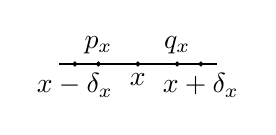
\begin{tikzpicture}
                \draw (0,0) -- (2,0);
                \draw[fill] (1,0) circle[radius=0.025] node[below]{$x$};
                \draw[fill] (0.2,0) circle[radius=0.025] node[below]{$x-\delta_x$};
                \draw[fill] (1.8,0) circle[radius=0.025] node[below]{$x+\delta_x$};
                \draw[fill] (0.5,0) circle[radius=0.025] node[above]{$p_x$};
                \draw[fill] (1.5,0) circle[radius=0.025] node[above]{$q_x$};
            \end{tikzpicture}
    \end{itemize} \hfill \qed
\end{dd}

\begin{lem}
    Niech $[a,b] \subseteq \bigcup\limits_{n=1}^\infty (a_n,b_n)$, wtedy istnieje $N \in \mathbb{N}$, t. że $\bigcup\limits_{n=1}^N (a_n,b_n) \supseteq [a,b]$.
    \begin{dd}
        $S = \{ x: a \le x \le b$, przedział $[a,x]$ przykrywa się skończoną ilością $(a_n,b_n)\}$ \\
        $S \neq \emptyset$, bo $a \in S$. $S$ jest ograniczony z góry. Niech $s = \sup S$. \\
        $ s \in [a,b] \subseteq \bigcup\limits_{n=1}^\infty (a_n,b_n)$. \\
        Istnieje $n_0, s \in (a_{n_0},b_{n_0})$. Istnieje $x \in S \ a_{n_0} < x < s $. \\
        Istnieje $N \ [a,x] \subseteq \bigcup\limits_{n=1}^N (a_n,b_n).$ \\
        $[a,s] \subseteq \bigcup\limits_{n=1}^{N'} \quad N' = \max(N,n_0)$ \\
        Zostało pokazać, że $s = b$. Można to zrobić w podobny sposób.
    \end{dd}
\end{lem}

\begin{wn}
    Dla $a \le b$ przedział $[a,b]$ jest zwarty, to znaczy z każdego pokrycia $[a,b]$ zbiorami otwartymi, 
    można wybrać pokrycie skończone.
\end{wn}

\begin{wn}
    Jeżeli $f: \mathbb{R} \rightarrow \mathbb{R}$ jest ciągła, to $f$ jest ograniczona na $[a,b]$.
\end{wn}
\begin{dd} 
    $[a,b] \subseteq f^{-1}[\mathbb{R}]  = \bigcup\limits_{n=1}^\infty f^{-1}[(-n,n)]$. 
    Z zwartości istnieje $n_0$, takie, że $[a,b] \subseteq f^{-1}[(-n_0,n_0)]$.
\end{dd} 

\begin{tw} 
    Każdy ciąg $x_n \in [0,1]$ ma podciąg zbieżny. 
\end{tw} 
\begin{dd} 
    Pokażemy, że istnieje $a \in [0,1]$, takie, że dla dowolnego 
    $\delta > 0, \ x_n \in (a-\delta,a+\delta)$ dla nieskończone wielu n. \\
    Wtedy dla $\forall k \in \mathbb{N} \ \exists n_k > n_{k-1} \quad x_{n_k} \in (a-\frac{1}{k},a+\frac{1}{k}).$ \\ 
    Załóżmy nie wprost, że $\forall a \in [0,1] \ \exists \delta_a > 0 \ (a-\delta_a,a+\delta_a)$ 
    zawiera skończenie wiele wiele wyrazów ciągu. \\
    $[0,1] \subseteq \bigcup\limits_{a \in [0,1]} (a-\delta_a,a+\delta_a) $. 
    Ze zwartości $[0,1] \subseteq \bigcup\limits_{n=1}^K (a_i-\delta_{a_i},a_i+\delta_{a_i}) $. \lightning \\ 
    (po lewej zawiera wszystkie wyrazy ciągu, po prawej tylko skończenie wiele)
\end{dd}

\begin{tw} 
    $\mathbb{R}$ jest spójna, to znaczy nie istnieje podział prostej na dwa zbiory otwarte rozłączone.
\end{tw} 
\begin{dd}
    Niech $U,V \neq \emptyset,$ otwarte, $ U \cap V = \emptyset, \ U \cup V = \mathbb{R}$.
    Niech $a \in U, \ b \in V, s = \sup (U \cap [a,b])$. \\ Skoro $s \in U$, to istnieje $\delta > 0$, 
    taka, że $(s-\delta,s+\delta) \subseteq U$, sprzeczność z definicją supremum.
\end{dd}
\section{Metryka i norma}
Niech X będzie przestrzenią liniową.
\begin{df} 
    \underline{Normą} na X nazywamy funkcję $\norm{\cdot}: X \rightarrow [0,\infty)$, spełniającą: 
    \begin{itemize} 
        \item[(N1)] $\norm{x} = 0 \Leftrightarrow x = 0\footnotemark$
        \item[(N2)] $\norm{a\cdot x} = |a| \cdot \norm{x} \qquad a \in K, x \in X$ (jednorodność)
        \item[(N3)] $\norm{x+y} \le \norm{x} + \norm{y} \qquad x,y \in X$ (nierówność trójkąta)
    \end{itemize} 
\end{df} 
    \footnotetext{Chodzi o 0 przestrzeni liniowej X}
\begin{uw}
    W przestrzeni unormowanej $(X,\norm{\cdot})$ wielkość $\norm{x-y}$ jest odległością $x$ do $y$.
\end{uw}
\begin{df} 
    \underline{Przestrzenią metryczną} nazywamy $(X,\rho)$, gdzie $\rho: X \times X \rightarrow [0,\infty)$ spełnia
    \begin{itemize} 
        \item[(M1)] $\rho(x,y) = 0 \Leftrightarrow x = y$
        \item[(M2)] $\rho(x,y) = \rho(y,x)$
        \item[(M3)] $\rho(x,y) \le \rho(x,z)+\rho(z,y)$
    \end{itemize} 
\end{df} 
\begin{uw}
    Jeżeli $(X,\norm{\cdot})$ jest p. unormowaną, to wzór $\rho(x,y) = \norm{x-y}$ określa metrykę na X.
\end{uw}

\begin{uw} 
    Dla danej przestrzeni metrycznej $(X,\rho)$ i $Y \subseteq X$, to $(Y,\widetilde\rho)$, gdzie $\widetilde\rho \neq \rho |_{Y \times Y}$.
\end{uw}
\begin{ozn}
    W p. metrycznej $(X,\rho)$ zbiór $B_r(X) = \{y \in X: \rho(x,y) < r\}$ nazywamy kulą o środku $x$ i promieniu $r \ (r > 0)$.
\end{ozn}
\begin{df} ~\newline
    Zbiór $U \subseteq X$ jest \underline{otwarty}, jeśli $\forall x \in U \ \exists \delta > 0, \ B_\delta (x) \subseteq U$. \\ 
    Zbiór $F \subseteq X$ jest \underline{domknięty}, gdy $X \setminus F$ jest otwarty ($\forall x \notin F \ \exists \, \delta > 0 \ B_\delta(x) \cap F = \emptyset$).
\end{df} 
\begin{df} 
    Dla dowolnego $A \subseteq X$ definiujemy $\overline{A}$:
    \[ x \in \overline{A} \Leftrightarrow \forall \delta > 0 \quad B_\delta(X) \cap A \neq \emptyset \]
\end{df} 

\begin{tw} 
    W dowolnej p. metrycznej $(X,\rho)$: 
    \begin{enumerate}[(1)]
        \item $A \subseteq X$ jest dokmnięty $\Leftrightarrow \ A = \overline{A}$ 
        \item $\overline{A}$ jest najmniejszym zbiorem domkniętym zawierającym A
        \item \begin{itemize}
            \item Jeżeli $A \subseteq B$ to $\overline{A} \subseteq \overline{B}$ 
            \item $\overline{A \cup B} = \overline{A} \cup \overline{B}$ 
            \item $\overline{A} = \overline{\overline{A}}$
            \end{itemize}
        \item Jeżeli $A,B$ są domknięte to $A \cup B$ jest domknięty. \\ 
            Jeżeli $A_t$ jest domknięty dla $t \in T$ to $\bigcap\limits_{t \in T} A_t$ jest domknięty.
    \end{enumerate}
\end{tw} 
\begin{dd} \hfill
    \begin{enumerate}[(1)] 
        \item Wynika z def.
        \item z (1) wiemy, że $\overline{A}$ jest domknięty oraz $A \overset{\text{def} \overline{A}}{\subseteq} \overline{A}$. Należy pokazać, że jeżeli $A \subseteq F$ to $\overline{A} \subseteq F$ i $F$ domknięty. \\ 
        Zał, że $A \subseteq F$ i $F$ jest domknięty. Niech $x \notin F$, istnieje $\delta$ t. że $B_\delta (x) \cap F = \emptyset$, wtedy $B_\delta (x) \cap A = \emptyset$, więc $x \notin \overline{A}$. 
    \end{enumerate}
    Pozostałe punkty zostawione na ćwiczenia. 
\end{dd} 

\begin{df} 
    Ciąg $(x_n)$ w przestrzeni metrycznej $(X,\rho)$ jest zbieżny do $x \in X$ jeżeli $\lim\limits_n \rho(x_n,x) = 0$.\\
    tzn. $\forall \ \varepsilon > 0 \ \exists N \ \forall n > N \ \rho(x_n,x) < \varepsilon$
\end{df} 

\begin{tw} 
    Dla zbioru $A \subseteq X$ NWSR: 
    \begin{enumerate}[(1)]
        \item A jest domknięty 
        \item dla dowolnego $(x_n)$, jeżeli $(x_n) \in A$ i $x_n \underset{n}{\rightarrow} x$, to $x \in A$.
    \end{enumerate} 
\end{tw} 
\begin{dd} Pozostawiony na ćwiczenia. \end{dd}

\section{Trochę o funkcjach ciągłych}
\begin{tw}[o ciągłości] 
    Niech $(X,\rho), (X',\rho ')$ będą p. metrycznymi. Dla $f: X \rightarrow X'$ NWSR:
    \begin{enumerate}[(i)]
        \item $\forall x \in X \ \forall \varepsilon > 0 \ \exists \delta > 0 \ \forall y \in X \quad \rho(x,y) < \delta \Rightarrow \rho'(f(x),f(y)) < \varepsilon$
        \item Dla dowolnego ciągu $(x_n) \ x_n \in X$, jeżeli $x_n \underset{n}{\rightarrow} x$, to $f(x_n) \underset{n}{\rightarrow} f(x)$
        \item Dla dowolnego $F \subseteq X'$ domkniętego $f^{-1}[F]$ jest domknięty w $X$.
        \item Dla dowolnego $V \subseteq X'$ otwartego $f^{-1}[V]$ jest otwraty w $X$.
    \end{enumerate}
\end{tw} 

\begin{dd} \hfill 
    \begin{itemize} 
        \item[(i) $\Rightarrow$ (ii)] Rozważmy $x_n \in X$ t. że $x_n \underset{n}{\rightarrow} x \in X$. 
        Chcemy pokazać, że $f(x_n) \underset{n}{\rightarrow} f(x)$, czyli $\forall \varepsilon > 0 \quad f(x_n) \subseteq B_\varepsilon (f(x))$ dla prawie wszystkich $n$.
        Dobieramy $\delta > 0$ tak jak w (i), wtedy, jeżeli $y \in B_\delta(x)$, to $f(y) \in B_\varepsilon (f(x))$. Skoro $x_n \underset{n}{\rightarrow} x$, 
        to $x_n \in B_\delta (x)$ dla prawie wszystkich $n$, więc $f(x_n) \subseteq B_\varepsilon (f(x))$ dla prawie wszystkich $n$.
        \item[(ii) $\Rightarrow$ (iii)] Rozważmy $F \subseteq X'$ domknięty. Chcemy pokazać, że $f^{-1}[F]$ jest domknięty w $X$. Rozważmy $x_n \in f^{-1}[F]$, zał. że jest zbieżny do $x$, Chcemy spr. że $x \in f^{-1}[F]$.
        Gdyby $x \notin f^{-1}[F]$ tzn $f(x) \notin F$. Istnieje $\varepsilon$ t. że $B_\varepsilon (f(x)) \cap F = \emptyset$. 
        Z zał. $f(x_n) \underset{n}{\rightarrow} f(x)$, czyli $f(x_n) \in F$ \lightning
        \item[(iii) $\rightarrow$ (iv)] weźmy $V \subseteq X'$ otwarty, wtedy $F = X' \setminus V$ - domknięty. $ f^{-1} [X' \setminus V]$ - domknięty, $f^{-1}[F]$ domknięty. \\
        A $f^{-1}[X' \setminus V] = X' - f^{-1}[V]$ jest domknięty, czyli $f^{-1}[V]$ otwarty. \lightning
        \item[(iv) $\rightarrow$ (i)] Ustalmy $x \in X$. Weźmy $\varepsilon > 0$. Szukamy $\delta > 0$ t. że jeżeli $\rho (x,y) < \delta \Rightarrow \rho ' (f(x),f(y)) < \varepsilon$.
        $ V = B_\varepsilon (f(x))$ jest zbiorem otwartym, więc $f^{-1}[V]$ jest otwarty, ponieważ $x \in f^{-1}[V]$.
        Istnieje $\delta > 0$ t. że $B_\delta (x) \subseteq f^{-1}[V]$. \\
        $y \in B_\delta (x) \Rightarrow f(y) \in V = B_\varepsilon (f(x))$\\
        $\rho (x,y) < \delta \Rightarrow \rho'(f(y),f(x)) < \varepsilon$. \hfill \qed
    \end{itemize} 
\end{dd} 

\begin{tw} Złożenie funkcji ciągłych jest ciągłe \end{tw}
\begin{dd} 
    Niech $f: X \rightarrow X', \ g: X' \rightarrow X''$ będą ciągłe. $g \circ f: X \rightarrow X''$. Niech $V \subseteq X''$ będzie otwarty, wtedy $g^{-1}[V]$ jest otwarty w $X'$.
    $(g \circ f)^{-1}[V] = f^{-1}[g^{-1}[V]]$ jest otwarty w X. \hfill \qed
\end{dd} 

\begin{tw} Jeżeli $f,g: X \rightarrow \mathbb{R}$ są ciągłe, to $f+g$ i $f \cdot g$ też są ciągłe. \end{tw} 
\begin{dd} Z def. na ciągach \end{dd} 
\begin{tw} Funkcja $\rho(\cdot,x): X \rightarrow [0,\infty)$ jest ciągła. \end{tw} 
\begin{dd} $| \rho(y,x) - \rho(z,x)| \le \rho(y,z)$ \end{dd} 
\begin{ozn} Przestrzenią euklidesową nazywamy $(\mathbb{R}^d,\norm{\cdot}_2\footnotemark)$. \end{ozn}
\footnotetext{$ \norm{x}_2 = \sqrt{\sum\limits_{i=1}^d |x(i)|^2} $}
\begin{tw} W $\mathbb{R}^d$ ciąg $x_n = (x_n(1),x_n(2),\ldots,x_n(d))$ jest zbieżny do $x = (x(1),x(2),\ldots,x(d))$ wtedy i tylko wtedy gdy $\forall i \le d \ \lim\limits_n x_n(i) = x(i)$. \end{tw}
\begin{dd} na ćwiczeniach \end{dd}

\subsection{Zbiory gęste, przestrzeń ośrodkowa}

\begin{df} Zbiór $D \subseteq X$ jest gęsty, jeśli $\overline{D} = X$. \end{df}
\begin{uw} $\overline{D} = X \Leftrightarrow \ \forall r > 0 \ \forall x \ B_r(x) \cap D \neq \emptyset \Leftrightarrow \forall x \ \exists d_n \in D \ \rho(x,d_n) \underset{n}{\rightarrow} 0$ \end{uw}
\begin{df} $X$ jest przestrzenią ośrodkową (separable), jeżeli $X$ zawiera przeliczalny zbiór gęsty.\end{df}  
\begin{tw} Przestrzenie euklidesowe są ośrodkowe \end{tw} 
\begin{dd} $\mathbb{Q}^d \subseteq \mathbb{R}^d $ \end{dd} 
\begin{tw}(Weiestrassa) Jeżeli $f \in C[a,b]$ to dla każdego $\varepsilon > 0$ istnieje wieloman $P$, taki, że $|P(x)-f(x)| < \varepsilon$ \end{tw}
\begin{wn} Zbiór wielomianów jest gęsty w $C[a,b]$ \end{wn} 
\begin{wn} Przestrzeń $C[a,b]$ jest ośrodkowa \end{wn}
\begin{dd} 
    Niech $A = \{P : P(x) = a_0 + a_1 x + \ldots + a_n x^n, n \in \mathbb{N} , \{a_n\} \in \mathbb{Q} \}$. $A$ jest gęsty w $C[a,b]$. \\ 
    Niech $f \in C[a,b]$ i $ \varepsilon > 0$. Z tw. Weiestrassa istnieje wieloman $W$, t. że $\forall x \ |W(x) - f(x)| < \frac{\varepsilon}{2}$.
    $W(x) = b_0 + b_1 x + \ldots + b_n x^n, \quad b_n \in \mathbb{R}$. Niech $M = max\{|a|,|b|\}$. Bierzemy $p(x) = a_0 + a_1 x + \ldots + a_n x^n$,t. że: 
    \begin{align*}
        a_0 \in \mathbb{Q} \quad |b_0 - a_0| &< \frac{\varepsilon}{2(n+1)}\\ 
        a_1 \in \mathbb{Q} \quad |b_1 - a_1| &< \frac{\varepsilon}{2(n+1)M} \\ 
        \vdots
    \end{align*}
    Wtedy $\norm{W-p}_\infty < \frac{\varepsilon}{2}$, czyli $\norm{p-f} < \varepsilon$ \hfill \qed  
\end{dd} 
\begin{uw} Przestrzeń ośrodkowa nie zawiera nieprzeliczalnej rodziny rozłącznych kul. \end{uw} 

\section{Baza Topologii} 
Topologia to rodzina wszystkich zbiorów otwartych. 
\begin{df} W przestrzeni $X$ rodzina zbiorów otwartych $\mathcal{B}$ jest bazą topologiczną, jeżeli dla dowolnego otwartego $U \subseteq X$ i $x \in U$ istnieje $B \in \mathcal{B}, x \in B \subseteq U$. \end{df}
\begin{tw} Przestrzeń metryczna jest ośrodkowa $\Leftrightarrow X$ ma przeliczalną bazę. \end{tw}
\begin{dd}\hfill 
    \begin{itemize} 
        \item[$\Rightarrow$] Niech $A \subseteq X$ będzie przeliczalny, gęsty. 
            $B = \{B_q(a): a \in A, q \in \mathbb{Q}\}$. Niech $U \subseteq X$ będzie otwarty i $x \in U$.
            Istnieje $\delta > 0$ t. że $B_\delta(x) \subseteq U$. 
            Z gęstości $A: \ A \cap B_{\frac{\delta}{2}} \neq \emptyset$. Wtedy 
            $\rho(a,x) < \frac{\delta}{2}$. Dobieramy $q \in \mathbb{Q} \ \rho(a,x) < q < \frac{\delta}{2}$. Wtedy 
            $x \in B_q(a)$ oraz $B_q(a) \subseteq B_\delta (x)$
        \item[$\Leftarrow$] Niech $\mathbb{B} = \{ B_1,B_2,\ldots\}$\footnotemark. Niech $B_n \neq \emptyset$. Wybieramy $a_n \in B_n.\ A = \{a_1,a_2,\ldots\}$ jest gęsty. 
    \end{itemize} 
\end{dd} 
\footnotetext{chodzi o kule o kolejnych promieniach}

\begin{df} Przestrzenie metryczne $(X,\rho), \ (X',\rho')$ są homeomorficzne, jeżeli istnieje $f: X \xrightarrow[1-1]{\text{na}} X'$, t. że
$f: X \rightarrow X'$ oraz $f^{-1}: X' \rightarrow X$ są funkcjami ciągłymi.\end{df}

\begin{df} Metryki $\rho_1$ i $\rho_2$ na $X$ są równoważne, jeżeli wyznaczają te same zbiory otwarte (tę samą topologię). \end{df} 
\begin{tw} Metryki są równoważne $\Leftrightarrow \ \rho_1$ i $\rho_2$ wyznaczają te same ciągi zbieżne. \end{tw}
\begin{ozn} Własność topologiczna jest niezmiennikiem homeomorfizmu \end{ozn}
\section{Własności metryczne}
\subsection{Zwartość}
\begin{df} Przestrzeń metryczna $X$ jest zwarta, jeżeli z każdego pokrycia $X$ zbiorami otwartmi można wybrać podpokrycie skończone. \\
    Zbiór $A \subseteq X$ jest zwarty jeżeli dla dowolnej rodziny $\{U_t : t \in T\}$ zbiorów otwartych w X, z faktu, że $A \subseteq \bigcup\limits_{t \in T} U_t$,
    wynika, że $A \subseteq U_{t_1} \cup U_{t_2} \cup \ldots \cup U_{t_n}$ dla pewnych $t_1,\ldots,t_n \in T$. \end{df}
\begin{tw} Dla przestrzeni metrycznej $X$ NWSR:
    \begin{enumerate}[(i)]
        \item Z każdego pokrycia otwartego $X$ można wybrać podpokrycie skończone.
        \item Z każdego pokrycia przeliczalnego $X$ można wybrać podpokrycie skończone. 
        \item dla każdego ciągu $(x_n)$ w $X$ istnieje $x \in X$ i $n_1 < n_2 < n_3 < \ldots$ t. że $\lim\limits_{k \rightarrow \infty} x_{n_k} = x$
    \end{enumerate} 
\end{tw}
\begin{dd} \hfill
    \begin{itemize}
        \item[(i) $\Rightarrow$ (ii)] oczywiste
        \begin{lem}
            Jeżeli $F_n \subseteq X \ F_n$ - domknięte, $\bigcap\limits_{i=1}^n F_i \neq \emptyset$, to $\bigcap\limits_{n=1}^\infty F_n \neq \emptyset$.
            \begin{dd} 
                Zał. że $\bigcap\limits_{n=1}^\infty F_n = \emptyset$. \\ 
                $ X = \bigcup\limits_{n=1}^\infty (X \setminus F_n) \overset{\text{z (ii)}}{=} \bigcup\limits_{n=1}^n(X \setminus F_i) = \bigcap\limits_{i=1}^n F_n = \emptyset$ \lightning
            \end{dd}
        \end{lem} 
        \item[(ii) $\Rightarrow$ (iii)] 
            Niech $x_n \in X, \ F_n = \overline{\{x_{n+1},x_{n+2},\ldots\}}. \ F_1 \supseteq F_2 \supseteq \ldots \supseteq F_n \neq \emptyset$.\\
            Z lematu istnieje $x \in \bigcap\limits_{i=1}^\infty F_i$. Zdefinnujmy $n_1 < n_2 < \ldots < n_k < \ldots, \quad \rho(x_{n_k},x) < \frac{1}{k}$. \\
            Dla danych $n_1 < \ldots < n_k \quad x \in F_{n_k} = \overline{\{x_{n_k+1},x_{n_k+2},\ldots\}}$, czyli $B_{\frac{1}{k}}(x) \cap \{x_{n_k+1},\ldots\} \neq \emptyset$, 
            więc $x_{n_k} \in B_{\frac{1}{k}}(x)$.
        \begin{lem} 
            Jeżeli przestrzeń $X$ spełnia wzór (iii) to $X$ jest ośrodkowa (ma bazę przeliczalną).
            \begin{dd} 
                Rozważmy $A \subseteq X$ taki, że $x,y \in A x \neq y$ to $\rho(x,y) \ge 1$. Wtedy $A$ jest skończony. Gdyby $A$ 
                zawierał $(x_n)$ t. że $(x_n \neq x_k)$ to ciąg $(x_n)$ nie zawierałby podciągu zbieżnego.
                Niech $A_n$ będzie maksymalnym zbiorem w $X$ t. że $x,y \in A_n \Rightarrow \rho(x,y) \ge \frac{1}{n}. A_n$ skończony. 
                $D = \bigcup\limits_{n=1}^\infty A_n$ - przeliczalny. $X = \overline{D}. D \cap B_\delta(x) \neq \emptyset$
            \end{dd} 
        \end{lem}
        \item[(iii) $\Rightarrow$ (i)] Wiem, że $X$ ma przeliczalnę bazę. W przestrzeni z przeliczalną bazą, jeżeli $X = \bigcup\limits_{t \in T}U_t$ jest pokryciem otwarty, 
            to istnieje przeliczalny $T_0 \subseteq T \  X = \bigcup\limits_{t \in T_0} U_t$. Wystarczy pokazać (iii) $\Rightarrow$ (ii). \\ 
            Przypuścmy, że $X = \bigcup\limits_{n=1}^\infty U_n, \ U_n$ otwarte, ale $\bigcup\limits_{i=1}^n U_i \neq X$. Niech $x_n \in X \setminus \bigcup\limits_{i=1}^n U_i$,
            wtedy $(x_n)$ nie ma podciągu zbieżnego. Niech $x \in X$, wtedy $x \in U_{n_0}$ otwarta, czyli istnieje $\delta$, t. że $B_\delta(x) \subseteq U_{n_0}$. \\ 
            $n > n_0 \Rightarrow x_n \notin B_\delta(x)$ czyli prawie wszystkie wyr $(x_n)$ są daleko. 
            \hfill \qed
    \end{itemize} 
\end{dd} 

\begin{tw} \hfill 
    \begin{enumerate}[(1)]
        \item Jeżeli $X$ jest przestrzenią metryczną zwartą i $Y \subseteq X$ jest domknięta to $Y$ jest zwarta.
        \item Jeżeli $Y$ jest p. zwartą i $Y \subseteq X$ to $Y$ jest domknięte w $X$. 
        \item Jeżeli $f: X \underset{\text{na}}{\rightarrow} Y$ jest ciągłą suriekcją na p. zwartej $X$, to $Y$ jest p. zwartą.
    \end{enumerate} 
\end{tw} 
\begin{dd} \hfill  
    \begin{enumerate}[(1)] 
        \item $Y \subseteq \bigcup\limits_{t \in T} U_t,\  U_t \in X$ otwarte. Wtedy $X = \bigcup\limits_{t \in T} U_t \cup ( X \setminus Y)$
        Ze zwartości $X \subseteq U_{t_1} \cup \ldots \cup \subseteq U_{t_n} \cup (X \setminus Y)$, wtedy $Y \subseteq U_{t_1} \cup \ldots \cup \subseteq U_{t_n}$. 
        \item Zał, że $Y$ nie jest domknięty. Istnieje $x \notin Y$, ale $ x = \lim\limits_n y_n, \ y_n \in Y$. Ciąg $y_n$ nie ma podciągu zbieżnego w $Y$. \lightning
        \item $f: X \underset{\text{na}}{\rightarrow} Y$. Niech $Y = \bigcup\limits_{t \in T} V_t, \ V_t$ - otwarte, wtedy $X = \bigcup\limits_{t \in T} \overbrace{f^{-1}[V_t]}{\text{otwarte}}$.
        $X = \bigcup\limits_{n=1}^k f^{-1}[V_{t_n}]$, czyli $Y = \bigcup\limits_{n=1}^k V_{t_n}$.
    \end{enumerate}
\end{dd}
\begin{tw} 
    Niech $(X_1,\rho_1),\ (X_2,\rho_2)$ będą zwarte. Rozważmy na $X_1 \times X_2$ metrykę $\rho$, t. że
    zbieżność w $\rho$ jest równoważna zbieżnosci "po współrzędnych". Wtedy $X_1 \times X_2$ jest zwarta.
\end{tw} 
\begin{dd} 
    Weżmy $(x_n). \ x_n = (x_n(1), x_n(2)) \subseteq X_1 \times X_2$. Mamy $x_n(1) \in X_1. \ X_1$ - zwarta, czyli $x_{n_k}(1) \underset{n}{\rightarrow} x(1)$. 
    $x_{n_k} \in X_2. \ X_2$ - zwarta, czyli $x_{n_{k_l}} \underset{n}{\rightarrow} x(2)$. 
\end{dd} 
\begin{tw} W przestrzeni euklidesowej $\mathbb{R}^d, \ A \subseteq \mathbb{R}^d$ jest zwarty $\Leftrightarrow A$ jest domknięty i ograniczony. \end{tw} 
\begin{dd}\hfill 
    \begin{itemize} 
        \item[$\Rightarrow$] Jeżeli $A$ jest zwarty, to $A$ jest domknięty (było) \\ 
            Jeżeli $A$ jest zwarty, to musi być ograniczony
        \item[$\Leftarrow$] $A \subseteq \mathbb{R}^d$ \\ 
            $ A \subseteq [-M,M]^d$ dla pewnego $M$. $[-M,M]$ jest zwarty, więc $[-M,M]^d$ jest zwarty. 
            $A$ jest domknięty, stąd $A$ jest zwarty.
    \end{itemize} 
\end{dd} 
\begin{wn} Jeżeli $X$ jest p. metryczną zwartą i $f: X \rightarrow \mathbb{R}$ jest ciągła to $f$ jest ograniczona i osiąga swoje kresy. \end{wn}
\subsection{Zupełność} 
\begin{df} Ciąg $(x_n)$ w przestrzeni metrycznej $(X,\rho)$ jest ciągiem Cauchy'ego jeżeli $\forall \varepsilon \ \exists N \ 
    \forall n, k > N \ \rho(x_n,x_k) < \varepsilon$. \\ 
    Metryka jest zupełna, jeżeli każdy ciąg Cauchy'ego jest zbieżny. \end{df} 
\begin{tw} Przestrzeń euklidesowa $\mathbb{R}^d$ jest zupełna \end{tw} 
\begin{dd} 
    Dla $d=1$ wynika z aksjomatu Dedekina. \\
    Niech $(x_n)$ będzie ciągiem Cauchy'ego w $\mathbb{R}^d$. Dla każdego $ j \le d \ |x_n(j)-x_k(j) \le \norm{x_n - x_k}_2$. \\
    $(x_n(j))$ jest ciągiem Cauchy'ego na $\mathbb{R}$. Stąd $x(j) = \lim\limits_n x_n(j)$ jest dobrze określone. \\
    $x = (x(1),x(2),\ldots,x(d)) = \lim\limits_n x_n$ \hfill \qed
\end{dd} 
\begin{tw} Dla dowolnej p. metrycznej $(X,\rho)$ przestrzeń $C_b(x)$ jest zupeła w metryce zbieżności jednostajnej (czyli $\norm{\cdot}_\infty$) \end{tw} 
\begin{dd} Niech $(f_n)$ będzie ciągiem Cauchy'ego w $C_b(x)$. \\ 
    Dla ustalonego $x \in X \ |f_n(x) - f_k(x)| \le \norm{f_n-f_k}_\infty$, więc $(f_n(x))$ jest ciągiem Cauchy'ego w $\mathbb{R}$. \\ 
    $f  \overset{\text{def}}{=} \lim\limits_n f_n$. Musimy spr. że $\norm{f_n-f} \underset{n}{\rightarrow} 0$ oraz $f \in C_b(x)$. \\
    Dla $\varepsilon > 0$ istnieje N, ,że $|f_k(x) - f_n(x)| < \varepsilon$ dla wszystkich $x \in X \ n,k > N$.
    Niech $k \rightarrow \infty, \ |f_n(x)-f(x)| < \varepsilon$ dla wszystkich $x \in X$, czyli $\norm{f_n-f} \le \varepsilon$ dla $n > N$.
    Druga część dowodu na ćwiczeniach. \hfill \qed
\end{dd}

\begin{tw} Jeżeli $(X,\rho)$ jest przestrzenią zupełną i $Y$ jest podprzestrzenią $X$, to $Y$ jest 
    zupełna w metryce $\rho \Leftrightarrow Y$ jest domknięta.
\end{tw}
\begin{dd} \hfill 
    \begin{itemize} 
        \item[$\Leftarrow$] Zał, że $Y$ jest domknięta. Niech $(y_n)$ będzie ciągiem Cauchy'ego w $Y$. 
            Ale wtedy $(y_n)$ jest ciągiem Cauchy'ego w $X$, zatem z zupełności $X$, istnieje $y \in X$ takie, że
            $ y= \lim\limits_n y_n$. Ale wtedy z domknniętości $Y \ y \in Y$.
        \item[$\Rightarrow$] Niech $y_n \in Y, \ x = \lim\limits_n y_n$ Chcemy sprawdzić, że 
            $x \in Y$. Skoro $y_n$ jest zbieżny to spełnia warunek Cauchy'ego. $Y$ jest zupełna, więc $(y_n)$
            ma granicę $y \in Y$. Wtedy $x = y \in Y$ (bo ciąg ma tylko jedną granicę).
    \end{itemize} 
\end{dd} 
\begin{tw}[Banacha o odwozorowaniu zwężającym] Niech $(X,\rho)$ będzie przestrzenią metryczną zupełną 
    i niech $T: X \to X$ będize odwozorowaniem zwężającym, tzn istnieje $c < 1$, takie, że 
    $\forall x,y \in X \ \rho( T (x), T (y)) \le c \cdot \rho(x,y)$. Wtedy istnieje dokładnie 
    jeden punkt $x_0 \in X$, taki, że $ T (x_0) = x_0$.
\end{tw} 
\begin{uw} $T$ jest funkcją ciągła \end{uw} 
\begin{dd} 
    Niech $x_1 \in X$. Rozważmy ciąg $x_{n+1} =  T (x_n)$. \\ 
    Niech $M = \rho(x_1, T (x1)).$
    \begin{align*}
        \rho ( T (x_1), T( T (x_1))) &\le c \cdot \rho(x_1, (x_1)) = c \cdot M \\ 
        \rho ( T ^n (x_1), T ^ {n+1}(x_1)) &\le c \rho( T^{n-1} (x_1), T^n (x_1)) \\
        \rho( T ^ {n+1}(x_1), T ^ n (x_1)) &\le M \cdot c^n 
    \end{align*} 
    \[
        \rho( T^{n+k} (x_1), T^n (x_1)) \le \rho ( T ^{n+1} (x_1), T^n(x_1)) + 
    \rho ( T^{n+2}(x_1), T^{n+1}(x_1)) + \ldots + \rho( T^{n+k}(x_1), T^{n+k-1}(x_1)) \le \]
    \[\le M(c^n + c^{n+1} + \ldots + c^{n+k-1}) < M \frac{c^n}{1-c} \]
    \[ \forall n \ \forall k > 0 \ \rho( T^{n+k}(x_1), T ^n(x_1)) \le 
    \overscript{\frac{M c^n}{1+c}}{\downarrow}{\text{dowolnie małe}} \]
    Ciąg $( T^n (x_1))_n$ jest ciągiem Cauchy'ego (zatem ma granicę bo jesteśmy w przestrzeni metrycznej zupełnej).
    Niech $x_0 = \lim\limits_n ( T^n (x_1))$. Wtedy $ T(x_0) = \lim\limits_n  T^{n+1}(x+1) = x_0$. \\ 
    Jeżeli $x_0 = T(x_1)$ oraz $\tilde x_0 = T(\tilde x_0) \ \rho(T(\tilde x_0),T(x_0)) \le c \rho(\tilde x_0,x_0)$. 
    Ponieważ $c < 1$, to $\rho(\tilde x_0,x_0) = 0$, czyli $\tilde x_0 = x_0$. \hfill \qed 
\end{dd} 
\begin{tw} 
        Niech $(X,\rho)$ będzie przestrzenią metryczną. NWSR: 
        \begin{enumerate}[(1)]
            \item Metryka $\rho$ jest zupełna
            \item Jeżeli $F_1 \supseteq F_2 \supseteq \ldots \supseteq F_n \supseteq \ldots$, gdzie $F_n$ 
                są domknięte i niepuste oraz $\operatorname{diam}_\rho (F) \to 0$, to $\bigcap\limits_{n=1}^\infty F_n \neq 0$.
        \end{enumerate} 
        \footnotetext{$\operatorname{diam}_\rho(A) = \sup\limits_{x,y \in A} \rho(x,y)$}
\end{tw} 
\begin{dd} \hfill 
    \begin{itemize} 
        \item[$(1) \Rightarrow (2)$] Niech $x_n \in F_n$. Wtedy $(x_n)$ spełnia warunek Cauchy'ego, bo dla 
            $k > 0 \ \rho(x_k,x_n) \le \operatorname{diam}_\rho (F_n) \to 0$. \\ 
            Niech $x = \lim\limits_n x_n$. Wtedy $x \in \bigcap\limits_{n=1}^\infty F_n$.
        \item[$(2) \Rightarrow (1)$] Niech $(x_n)$ spełnia warunek Cauchy'ego. 
            $F_n = \overline{\{x_{n+1},x_{n+2},\ldots\}} \ \operatorname{diam}_\rho (F_n) \to 0$ \\
            $x \in \bigcap\limits_{n=1}^\infty F_n$. Wtedy $x = \lim\limits_n x_n$.
    \end{itemize} 
\end{dd} 
\begin{tw} (Baire'a o kategorii) Jeżeli $X$ jest p. metryczną zupełną, $F_n \subseteq X$ są domknięte i $\operatorname{int}(F_n) = \emptyset$,
to $\bigcup\limits_{n=1}^\infty F_n \neq X$. \end{tw} \begin{dd} Definiujemy indukcyjnie ciąg $x_n \in X$ i $r_u > 0$, tak aby: 
    \begin{itemize} 
        \item $B_{r_n}(x_n) \cap (F_1 \cup \ldots \cup F_n) = \emptyset$
        \item $B_{r_{n+1}}(x_{n+1}) \subseteq B_{r_n}(x_n) $
        \item $\lim\limits_n r_n = 0$
    \end{itemize} 
    Z zupełności istnieje $x \in \bigcap\limits_{n=1}^\infty \overline{B_{r_n}(x_n)}$. Wtedy 
    $x \notin \bigcap\limits_{n=1}^\infty F_n$. 
\end{dd} 
\begin{tw} (Baire'a) W p. zupełnej $X$ suma $\bigcup\limits_{n=1}^\infty F_n$ zbiorów domkniętych o pustym wnętrzu ma puste wnętrze. \\ 
    \textbf{Dualnie}, jeżeli $G_n \subseteq X$ są otwarte i gęste to $\bigcap\limits_{n=1}^\infty G_n$ jest gęsty.
\end{tw} 
\begin{dd} 
    Niech $U \subseteq X$ będzie otwarty, $U \neq \emptyset$. \\ 
    $B_r(y) \subseteq U$ dla $y \in X,\ r > 0$ \\
    $B_s(z) \subseteq \overline{B_s(z)} \subseteq B_r(y)$ \\ 
    $x_0 = \overline{B_s(z)} \leftarrow$ teraz stosujemy tę samą konstrukkcję jak w poprzednim dowodzie.
\end{dd} 
\begin{df} ~\\
    Zbiór $ A \subseteq X$ jest nigdziegęsty, jeżeli $\operatorname{int}(\overline{A}) = \emptyset$ \\
    Zbiór $A \subseteq X$ jest brzegowy, jeżeli $\operatorname{int}(A) = \emptyset$. \\ 
    Zbiór $A \subseteq X$ jest I-kategorii, jeżeli $A \subseteq \bigcup\limits_{n=1}^\infty B_n$, gdzie $B_n$ jest nigdziegęste.
\end{df} 
\begin{uw} Z tw. Baire'a przestrzeń metryczne zupełna nie jest I-kategorii \end{uw}
\begin{df} (liczb Liouville'a)
    $$ x \in L \Leftrightarrow \forall n \ \exists q \ge 2, q \in \mathbb{N} \ \exists p \in \mathbb{Z} \ |x - \frac{p}{q}| < \frac{1}{q^n}. $$
    $x \in L \rightarrow x$ jest przestępna. \end{df}
    "Typowa" $x \in \mathbb{R}$ jest liczbą Liouville'a. $\mathbb{R} = L \cup \overbrace{\bigcup\limits_{n=1}^\infty F_n,}^{\text{I kategorii}} \ F_n$
    domknięte, $\operatorname{int}(F_n) = \emptyset$. 
    %chuj się odjebało ja pierdolę 
\section{Związki zwartości i zupełności} 
\begin{tw} Każda p. metrczyna zwarta jest zupełna \end{tw} 
\begin{dd} Niech $(x_n)$ będzie ciągiem Cauchy'ego. $X$ jest zwarta, więc istnieje $n_1 < n_2 < \ldots$ 
    i $x \in X, \lim\limits_{k \to \infty} x_{n_k} = x$. Sprawdzamy, że wtedy $\lim\limits_{n \to \infty} x_n = x$. 
    $$ \rho(x_n,x) < \rho(x_n,x_{n_k}) + \rho(x_{n_k},x) $$
    Ustalony $\varepsilon > 0$: 
    $$ \rho(x_{n_k},x) < \frac{\varepsilon}{2} \text{, dla } k \ge k_0$$
    $$\rho(x_n,x_{n_k}) < \frac{\varepsilon}{2} \text{, dla } n,n_k > N \text{, czyli}$$
    $$\rho(x_n,x) < \varepsilon \text{, dla wszystkich n}$$
    \hfill \qed
\end{dd} 
\begin{df} P. metryczna $(X,\rho)$ jest całkowicie ograniczona, jeżeli dla każdego $\varepsilon > 0$ istnieje 
    $n$ i $x_1,\ldots,x_n \in X$ takie, że $X = \bigcup\limits_{i=1}^n B_\varepsilon(x_i)$.
\end{df}
\begin{uw} Stwierdzenie w p. metrycznej $X$ zbiór $A \subsetneq X$ jest zwarty $\Leftrightarrow$ A domknięty i ograniczony jest GŁĘBOKO BEZ SENSU. \end{uw}
\begin{tw} Przestrzeń metryczna $(X,\rho)$ jest zwarta wtedy i tylko wtedy gdy jest zupełna i całkowicie ograniczona. \end{tw} 
\begin{dd} \hfill 
    \begin{itemize} 
        \item[$\Rightarrow$] Zał. że $X$ jest zwarta. Wtedy jest zupełna (było). \\ 
        $\varepsilon > 0 \ quad X = \bigcup\limits_{x \in X} B_\varepsilon(x)$. Ze zwartości istnieje pokrycie skończone, 
        a więc istnieje $n$ i $x_1,\ldots,x_n \in X, \ X = \bigcup\limits_{i=1}^n B_\varepsilon(x_i)$. 
        \item[$\Leftarrow$] Rozważmy $(x_n)$ w $X$. Z całkowitej ograniczoności dla każdego $k \in \mathbb{N}$,
            istnieją $z_1,\ldots,z_m \bigcup\limits_{i=1}^m B_{\frac{1}{k}}(z_i) = X$. 
            Istnieją, więc kule $A_k$ o promieniu $\frac{1}{k}$ takie, że $A_1 \supseteq A_2 \subseteq \ldots$, 
            takie, że dla każdego $k, \ x_n \in A_k$ Dla nieskończenie wielu $n$.
            Niech $x \in \bigcup\limits_{k=1}^\infty \overline{A_k}$. Wtedy dla każdego 
            $k$, $\rho(x_n,x) < \frac{1}{k}$ dla nieskończenie wielu $n$. Wtedy istnieje $n_1 < n_2 < 
            \ldots < n_j < \ldots < \rho(x_n,x) < \frac{1}{j}$ 
        \hfill \qed
    \end{itemize} 
\end{dd}
%%%%%%%%%%%%%%%%%%%%%%%%%%%%%%%%%%%%%%%%%%%%%%%%%%%%%%%%%%
\textbf{DYGRESJA} $(\mathbb{Q},| \cdot |) \underset{\text{uzupełnienie}}{\rightsquigarrow}(\mathbb{R},| \cdot |)$
%%%%%%%%%%%%%%%%%%%%%%%%%%%%%%%%%%%%%%%%%%%%%%%%%%%%%%%%%
\begin{tw} Dla każdej p. metrycznej $(X,\rho)$ istnieje izometria $I: X \rightarrow \widetilde{X}$, gdzie
    $(\widetilde{X},\widetilde{\rho})$ jest przestrzenią metryczną zupełną i $I[X]$ jest gęsty w $\widetilde{X}$.
\end{tw} 
\begin{dd} Rozważamy przestrzeń metryczną zupełną $C_b(x)$ z metryką zadaną przez $\norm{\cdot}_\infty$. 
    Zdefiniujmy $I: X \rightarrow C_b(X)$, gdzie $I$ jest izometrią i $\widetilde{X} = \overline{I[X]}$ 
    i $\widetilde{\rho}$ będzie zadane przez $\norm{\cdot}_\infty$. \\ 
    Definiujemy $I, x \rightarrow I_x, \ I_x(y) = \rho(x,y)$ (to by działało przy założeniu $\rho$ ograniczone). \\
    $I_x(y) = \rho(x,y) - \rho(\alpha,y) \ quad \alpha \in X$ \\. 
    Przy ustalonym $x \ I_x(\cdot)$ zmiennej y jest ciągła i ograniczona, bo $|\rho(x,y)-\rho(a,y)| \le \rho(x,a)$. \\
    \textbf{Wniosek} $I_x \in C_b(x)$. \\ 
    $I : (X,\rho) \underset{\text{izometria}}{\to} (C_b(x),\norm{\cdot}_\infty) $. \\ 
    $x,x' \in X$. Mamy pokazać, że $\norm{I_x - I_{x'}}_\infty = \rho(x,x')$. \\ 
    $\norm{I_x - I_{x'}}_\infty = \sup\limits_{y \in X}|I_x(y) - I_{x'}(y)|=\sup\limits_{y \in X}
    |\rho(x,y)-\rho(a,y)-(\rho(x',y)-\rho(a,y)| = \sup\limits_{y\in X}|\rho(x,y)-\rho(x',y)| = \rho(x,x')$
    \hfill \qed
\end{dd} 
\begin{ft} (o przestrzeniach zwartych) \\
Jeżeli $X$ jest p. zwartą i $U$ jest pokryciem otwarty $X$, to istnieje $\delta > 0$, że dla 
dowolnego $x \in X$, $B_\delta(x)$ zawiera się w pewnym $u \in U$.
\end{ft} 
\begin{wn} Jeżeli $f: X \to \mathbb{R}$ jest ciągła na p. zwartej $X$, to 
    $f$ jest jednostajnie ciągła. Niech $\varepsilon > 0$. Dla dowolnego $x \in X$ istnieje otwarte otoczenie 
    $U_x \ni x$ takie, że
\end{wn}
\section{Współczynnik Lebesgue'a}
\begin{df} 
    Dana jest przestrzeń $X$ i pokrycia $U, V$ zbiorami otwartymi. $V$ jest wpisane w $U$ (jest drobniejsze, 
    subtelniejse), jeżeli 
    \[ \forall v \in V \ \exists u \in U \ v \subseteq u \]
\end{df} 
\begin{tw} 
    Jeżeli $X$ jest przestrzenią metryczną zwartą to dla dowolnego pokrycia $U$ zbiorami otwartymi 
    istnieje $\delta > 0$, taka, że $\{ B_\delta(x) : x \in X\}$ jest wpisane w $U$. 
\end{tw} 
\begin{dd} 
    \begin{gather*}
        \forall x \in X \exists u \in \mathcal{U} \ x \in u \\ 
        \text{stąd } \forall x \in X \ \exists \delta (x) > 0 \exists u \in U \ B_{2\delta (x)} \subseteq U \\
        \text{Wtedy } \{ B_{\delta (x)} (x) : x \in X \} \text{ jest pokryciem} X \\
        \text{Istnieje } n \in \mathbb{N} \text{ oraz } x_1,\ldots,x_n \in X \\ 
        \bigcup_{i=1}^n B_{\delta (x_i)} (x_i) = X \\ 
        \delta = \min_{i=1}^n \delta(x_i). \text{ Wtedy } \delta \text{ spełnia tezę}. \\ 
        \text{Niech } x \in X \ \exists i \le n \ x \in B_{\delta_i} (x_i) \text{, wtedy} \\ 
        B_\delta (x) \subseteq B_{2\delta_i} (x_i)
    \end{gather*} 
\end{dd} 
\begin{prz} 
    Jeżeli $X$ jest zwarta i $f : X \to Y$ jest funkcją ciągłą w przestrzeni metrycznej $Y$, to $f$ 
    jest jednostajnie ciągła. 
    \begin{enumerate}[(1)]
        \item Dla każdego $\varepsilon > 0, \ X $ można pokryć zbiorami otwartymi $u$, takimi, że $x,x' \in U 
            \Rightarrow \rho_Y (f(x),f(x')) < \varepsilon$.
        \item Współczynnik Lebesgue'a $\delta$ dla pokrycia z $(1)$ daje jednostajną ciągłość
    \end{enumerate} 
\end{prz}
\subsection{Kostka Hilberta $[0,1]^\mathbb{N}$}
    Niech $m$ będize metryką na $[0,1]^\mathbb{N}$, daną wzorem 
    \[ m(x,y) = \sum_{n=1}^\infty \frac{1}{2^n} |x(n) - y(n)| \ \text{(metryka kanoniczna)}\]
\begin{df} 
    Mówimy, że przestrzeń $X$ zanurza się w przestrzeni $Y$, jeżeli istnieje różnowartościowa
    $f: X \to Y$, która jest homeomorifzmem pomiędzy $X$ i $f[X]$.
\end{df} 
\begin{tw} 
    Dla p. metrycznej $(X,\rho)$ NWSR: 
    \begin{enumerate}[(a)]
        \item $X$ jest ośrodkowa 
        \item $X$ zanurza się w $[0,1]^\mathbb{N}$
    \end{enumerate} 
\end{tw} 
\begin{lem} 
    Ciąg $x_n \in [0,1]^\mathbb{N}$ jest zbieżny do $x \in [0,1]^\mathbb{N}$ wtedy i tylko wtedy, gdy 
    $\forall j \in \mathbb{N} \ \lim\limits_{n} x_n(j) = x(j)$.
    \begin{dd} \hfill 
        \begin{itemize} 
            \item[$\Rightarrow$] $m(x_n,x) = \sum\limits_{j=1}^\infty \frac{1}{2^j} |x_n(j) - x(j)| 
                    \ge \frac{1}{2^k} |x_n(k) - x(k)|$ \\ 
                    jeśli $m(x_n,x) \to 0$, to $ \forall k |x_n (k) - x(k)| \to 0$
                \item[$\Leftarrow$] Zał. że $\forall k \ \lim\limits_n x_n (k) = x(k)$ \\ 
                    Niech $\varepsilon < 0$, weźmy $N \ \frac{1}{2^N} < \frac{\varepsilon}{2}$. \\ 
                    $\exists n_0 \ \forall n > n_0 \forall j < N \ |x_n(j) - x(j)| < \frac{\varepsilon}{2}$ \\ 
                    Wtedy dla $n > n_0 \ m(x_n,x) < \varepsilon$.
        \end{itemize} 
    \end{dd} 
\end{lem}
\begin{uw} 
    Funkcja $F: X \to [0,1]^\mathbb{N}$ jest ciągła $\Leftrightarrow \ F=(f_1,f_2,\ldots,f_n,\ldots)$ i 
    $f_n : X \to [0,1]$ jest ciągła każdego $n$.
\end{uw} 
\begin{dd} \hfill
    \begin{itemize} 
        \item[$(b) \Rightarrow (a)$] Niech $x \simeq X' \subseteq [0,1]^\mathbb{N}$ \\ 
            $[0,1]^\mathbb{N}$ jest ośrodkowa więc ma przeliczalną bazę $B$.
            Wtedy $ \{ b \cap X' : b \in B \}$ stanowi przeliczalną bazę X'. 
            Stad $X$ ma przeliczalną bazę, więc jest ośrodkowa. 
        \item[$(a) \Rightarrow (b)$] Niech $D = \{x_1,x_2,\ldots\}$ będzie gęsty w $X$. 
            Bez starty ogólności, załóżmy, że $\rho (x,x') \le 1$ dla $x,x' \in X$.
            $f_n : X \to [0,1] \ f_n = \rho (x,x_n)$. Wtedy $f_n$ jest ciągła. \\ 
            $ F: X \to [0,1]^\mathbb{N}$ taka, że $F = (f_1,f_2,\ldots,f_n,\ldots)$ jest ciągła (z uwagi). \\
            $F$ jest $'1-1'$. $x,x' \in X, x \neq x'$ \\ 
            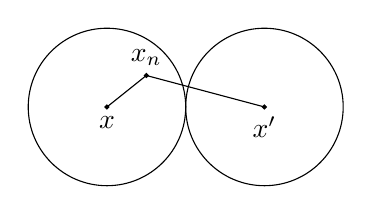
\begin{tikzpicture} 
                \draw (-1,0) circle[radius=1];
                \draw (1,0) circle[radius=1]; 
                \draw[fill] (-1,0) circle[radius=0.025] node[below]{$x$}; 
                \draw[fill] (1,0) circle[radius=0.025] node[below]{$x'$};
                \draw[fill] (-0.5,0.4) circle[radius=0.025] node[above]{$x_n$};
                \draw (-1,0) -- (-0.5,0.4); 
                \draw (-0.5,0.4) -- (1,0);
            \end{tikzpicture} 
            $f_n(x) \neq f_n (x')$ \\ 
            Mamy sprawdzić, że $F^{-1} : F[X] \to X$ jest ciągła. \\
            Jeżeli $F(y_j) \to F(y)$, to $y_j \to y$.
            Niech ciąg $(y_j)$ nie jest zbieżny do $y$. Istnieje $\varepsilon > 0 
            y_i \notin B_\varepsilon (y)$ dla nieskończenie wielu $j$. \\ 
            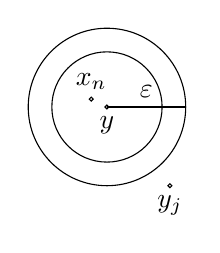
\begin{tikzpicture} 
                \draw circle[radius=1];
                \draw (0,0)--(1,0) node[midway,above]{$\varepsilon$}; 
                \draw circle[radius=0.025] node[below]{$y$};
                \draw (0.8,-1) circle[radius=0.025] node[below]{$y_j$};
                \draw circle[radius=0.7];
                \draw (-0.2,0.1) circle[radius=0.025] node[above]{$x_n$};
            \end{tikzpicture} \\ 
            Stad $F(y_j)$ nie zbiega do $F(y)$. Niech $x_n \in B_{\frac{\varepsilon}{3}} (y)$ \\
            $f_n (y) = \rho(y,x_n) < \frac{\varepsilon}{3}$ \\ 
            $f_n (y_j) = \rho(y_j,x_n) \ge \frac{2\varepsilon}{3}$ \\ 
            stąd $F(y_j)$ nie zbiega do $F(y)$ \lightning.
    \end{itemize} 
\end{dd} 

\begin{tw} Kostka Hilberta jest zwarta w metryce m. \end{tw} 
\begin{lem} 
    Jeżeli $\mathbb{N} \supseteq A_1 \supseteq \ldots \supseteq A_j \supseteq \ldots $ są nieskończone to 
    istnieje nieskończony $A \subseteq N$ taki, że $A \overset{\ast}{\subseteq} A_j$, czyli
    $A \setminus A_j$ jest skończony.
    \begin{dd} 
        Definujemy $n_1 < n_2 < \ldots < n_k < \ldots$ \\ 
        $n_k$ - pierwsza liczba ze zbioru $A_k$, która jest większa od $n_{k-1}$.
        $A = \{n_1,n_2,\ldots\}$ \hfill \qed
    \end{dd} 
\end{lem} 
\begin{dd} 
    Niech $x_n \in [0,1]^\mathbb{N}$. \\ 
    Pokażemy, że $(x_n)$ ma podciąg zbieżny. Istnieje nieskończony $A_1 \subseteq \mathbb{N}$ taki,  
    że $(x_n(1))_{n \in A_1}$ jest zbieżny do $x(1)$. Rozważmy $(x_n)_{n \in A_1}$. Istnieje 
    nieskończony $A_2 \subseteq A_1$, taki, że $(x_n (2))_{n \in A_2}$ jest zbieżny do $x(2)$. \\ 
    Definiujemy nieskończone zbiory $A_1 \supseteq A_2 \subseteq \ldots$ takie, że dla każdego 
    $j \ (x_n(j))_{n \in A_j}$ jest zbieżny do $x(j)$.
    Niech $A \overset{\ast}{\subseteq} A_j$ dla każdego $j$. Wtedy $(x_n)_{n \in A}$ jest zbieżny do 
    $x = (x(1),x(2),\ldots) \in [0,1]^\mathbb{N}$.
\end{dd} 

\begin{wn} \hfill 
    \begin{enumerate}[(1)]
        \item Każda przestrzeń metryczna ośrodkowa zanurza się w przestrzeni metrycznej zwartej
        \item Przestrzeń $X$ jest zwarta wtedy i tylko wtedy, gdy $X$ jest homeomorifczna z domkniętym
            podzbiorem $[0,1]^\mathbb{N}$.
        \item Ka każdej przestrzeni metrycznej ośrodkowej istnieje równoważna metryka całkowicie ograniczona.
    \end{enumerate}
\end{wn} 

\begin{dd} 
    \begin{enumerate}[(1)] 
        \item chyba oczywiste xD
        \item Jeżeli $X$ jest zwarta (i metryczna) to $X$ jest ośrodkowa, więc $X \hookrightarrow [0,1]^\mathbb{N}$. \\ 
            Istnieje $F: X \underset{'1-1'}{\xrightarrow{\text{ciągły}}} [0,1]^\mathbb{N}$. Wtedy 
            $F[X]$ jest zwarty, więc jest domknięty.
        \item Istnieje zanurzenie $F: X \to [0,1]^\mathbb{N}$. Metryka $m$ jest całkowicie ograniczona. \\ 
            Wtedy $\rho' (x,y) = m(F(x),F(y))$, definicjia równoważna metryce całkowicie ograniczonej.
    \end{enumerate} 
\end{dd} 
\begin{tw}[tw. Aleksandrowa]
    Dla danej przestrzeni metrycznej ośrodkowej $(X,\rho)$ NWSR: 
    \begin{enumerate}[(1)]
        \item Istnieje równoważna metryka zupełna
        \item $X$ jest homeomorficzna z pozdbiorem $[0,1]^\mathbb{N}$ typu $G_\delta$.
    \end{enumerate} 
\end{tw}
\begin{wn} Na $\mathbb{R} \setminus \mathbb{Q}$ istnieje metryka równoważna zupełna. \end{wn} 
\begin{prz} 
    $X = (0,1)$ nie jest zupełna w metryce euklidesowej, ale $\rho (x,y) = | \operatorname{arctg} x - \operatorname{arctg} y|$ jest 
    równoważna metryce zupełnej.
\end{prz} 
\begin{prz} 
    $X = \mathbb{Q}$ nie jest zuepłna w metryce euklidesowej. Dowolna metryka równoważna na $\mathbb{Q}$ nie jest zupełna. 
    $\mathbb{Q} = \bigcup\limits_{q \in \mathbb{Q}} (q)$
\end{prz}
\section{Topologia}
\begin{df} Przestrzenią topologiczną nazywamy parę $(X,\mathcal T)$, 
    gdzie $X \neq \emptyset,\ \mathcal T \subseteq \mathcal P (X)$, taka, że
    \begin{itemize} 
        \item $\emptyset,X \in T$
        \item $\mathcal T$ jest zamknięta na skoczone przkeroje 
        \item $\mathcal T$ jest zamknięta na dowolne sumy. 
    \end{itemize} 
    Zbiór $U \in \mathcal T$ nazywamy otwartym; Zbiór $F \subseteq X$ jest domknięty,
    jeżeli $X \setminus F \in \mathcal T$. 
\end{df} 
\begin{przy}\hfill
    \begin{enumerate}[(1)]
        \item $\mathcal T = \{ \emptyset, X \}$ jest topologią antydyskretną. 
        \item $\mathcal T = \mathcal P (X)$ topologia dyskretna. 
        \item Jeżeli $(X,\rho)$ jest przestrzenią metryczną, to $U \in \mathcal T 
            \Leftrightarrow \forall x \in U \ \exists \, \delta > 0 \ B_\delta (x) \in U$.
    \end{enumerate} 
\end{przy} 
\begin{df} 
    W przestrzeni topologicznej $(X,\mathcal T)$, rodzina $\mathcal B \subseteq \mathcal T$ jest bazą, jezeli 
    dla każdego $x \in X$ i $X \in U \in \mathcal T$ istnieje $B \in \mathcal B$, taki, że $x \in B \subseteq U$
\end{df}

\begin{tw} 
    Niech $\mathcal B \subseteq \mathcal P (x)$ będzie rodziną taką, że 
    \[ \forall B_1,B_2 \in \mathcal B \ \forall x \in B_1 \cap B_2 \ \exists B \in \mathcal B \ x \in B \subseteq 
    B_1 \cap B_2 \]
    Wtedy biorąc z $\mathcal T$ wszystkie możliwe sumy zbiorów z $\mathcal B$ otrzymujemy topologię na $X$.
\end{tw} 

\begin{df} W przestrzeni topologicznej $(X,\mathcal T)$ rodzinę $\mathcal B(x), \ x \in X$ nazywamy bazę
    w punkcie x, jeżeli dla każdego $U \in \mathcal T$, takiego, że $x \in U$ istnieje $B \in \mathcal B(x)$, że 
    $x \in B \subset U$.
\end{df} 

\begin{tw} 
    Jeżeli dla kazdego $x \in X$  wybierzemy rodziny $\mathcal B(x)$ (jako bazę lokalną)
    i spełniony będzie warunek 
    \[ \forall x \ \forall y \ \forall B \in \mathcal B(x) \ y \in B \Rightarrow 
    \exists B_1 \in \mathcal B(y) \ y \in B_1 \subseteq B \]
    to możemy zdefiniować topologię na $X$, przez 
    \[ U \in \mathcal T \Leftrightarrow \forall x \in U \exists \, B \in \mathcal B(x) \ x \in B \subseteq U \]
\end{tw} 
\begin{przy} \hfill
    \begin{enumerate}[(1)]
        \item $X = \mathbb R$ \\ 
            $\mathcal B = \{ (a,b): a < b \}$ jest bazą topoologii natrualnej \\ 
            $\mathcal B(x) = \{(x-\delta,x+\delta): \delta > 0 \}$ - baza lokalna w $X$.
        \item Niech $\mathcal B = \{[a,b]: a < b \}$ \\ 
            $\{ x\} = [x-1,x]\cap[x,x+1]$ jest otwarty \\ 
            $\mathcal T = \mathcal P (\mathbb R)$
        \item $\mathcal B = \{[a,b): a < b\}$ jest bazą topologii Sorgenfrey'a. $\mathbb R$ z tą 
            topologią nazywamy strzałką.
    \end{enumerate} 
\end{przy} 
\begin{df} 
    Przestrzeń topologiczna $(X,\mathcal T)$ jest metryzowalna jezeli istnieje metyrka $\rho$ na $X$ taka, że
    \[ U \in \mathcal T \Leftrightarrow \forall x \in U \exists \, \delta > 0 \ B_\delta (x) \subseteq U \]
\end{df} 
\begin{przy} \hfill
    \begin{enumerate}[(1)]
        \item $\rho (x,y) = |x-y|$
        \item $d(x,y) = \begin{cases} 1 & x \neq y \\ 0 &x = y \end{cases}$
        \item Strzałka nie jest metryzowalna. Przypuśćmy ,że metryka $\rho$ wyznacza topologię strzałki. 
            \[ \forall x \in \mathbb R \ \exists \, \delta(x) \ \forall y < x \ \rho (y,x) \ge \delta (x)\]
            \[ \mathbb R = \bigcup^\infty_{n=1} A_n, \quad A_n = \{ x \in \mathbb R : \delta(x) \ge \frac{1}{n} \} \]
            Z tw. Baire'a istnieje $n_0 \in \mathbb N$, takie, że $\operatorname{Int}(\overline{A_{n_0}}) \neq 
            \emptyset$. Istnieje $a < b, \ (a,b) \subseteq \overline{A_{n_0}}$. Tzn. zbiór 
            $A_{n_0}$ jest gęsty w $(a,b)$.\\[1cm]
            \begin{tikzpicture} 
                \draw (-5,0) -- (5,0); 
                \draw (-4.5,-0.1) -- (-4.5,0.1) node[above]{$a$};
                \draw (4.5,-0.1) -- (4.5,0.1) node[above]{$b$};
                \draw (-2,-0.2) -- (-2,0.2) node[above]{$y \in A_{n_0}$};
                \draw[fill] (0.5,0) circle[radius=0.025] node[below]{$x_1$};
                \draw[fill] (-0.8,0) circle[radius=0.025] node[below]{$x_2$};
                \draw[fill] (-1.3,0) circle[radius=0.025] node[below]{$x_3$};
                \draw[fill] (-1.75,0) circle[radius=0] node[below]{$\ldots$};
            \end{tikzpicture} \\[1cm] 
            Niech $x_k \in A_{n_0},\ x_1 > x_2 > \ldots > y,\ |x_k - y| < \frac{1}{k}$. 
            $\rho(x_k,y) \ge \frac{1}{n_0}$ \\ 
            $r > \frac{1}{n_0} \ B_r (y) \ni X_k$ dla prawie wszystkich $k$.
    \end{enumerate} 
\end{przy} 
\begin{df} 
    W przestrzeni topoligcznej $X$ definiujemy $\overline A,\ \operatorname{Int} A$ dla $A \subseteq X$
    \begin{gather*} 
        x \in \overline A \Leftrightarrow \forall U \in \mathcal T x \in U \Rightarrow U \cap A \neq \emptyset \\ 
        x \in \operatorname{Int} A \Leftrightarrow \exists U \in \mathcal T \ x \in U \subseteq A
    \end{gather*} 
\end{df} 
\begin{tw} 
    $\overline{A \cup B} = \overline A \cup \overline B$
\end{tw} 
\begin{dd} ~\\
    $C \subseteq D \Rightarrow \overline C \subseteq \overline D$ \\ 
    $A \subseteq A \cup B \quad B \subseteq A \cup B$ \\ 
    $\overline A \subseteq \overline{A \cup B} \quad \overline B \subseteq \overline{A \cup B}$ \\ 
    $\overline A \cup \overline B \subseteq \overline{A \cup B}$ \\ 
    Chcemy sprawdzić, że $\overline{A \cup B} \subseteq \overline A \cup \overline B$. \\ 
    Niech $x \neq \overline A \cup \overline B$. Wtedy
    \begin{tabular}[t]{l} 
    $x \notin \overline A$, więc istnieje $U \in \mathcal T,\ x \in U \quad U \cap A = \emptyset$ \\ 
    $x \notin \overline B$, więc istnieje $V \in \mathcal T,\ x \in V \quad V \cap B = \emptyset$ \\ 
    $W = U \cap V$. Wtedy $W$ jest otoczeniem $x$ tj. \\ 
    $W \ni X, \ W \in \mathcal T, \ W \cap (A \cup B) = \emptyset,
    \ x \notin \overline{A \cup B}$
    \hfill \qed
    \end{tabular}
\end{dd} 
\begin{przyp} 
    W przestrzeni metrycznej $(X,\rho)$ 
    \[ x \in \overline A \Leftrightarrow \text{istnieje } a_n \in A \text{, że} \lim_n a_n = x \]
    W przestrzeni topologicznej $X$ definiujemy zbieżność $(x_n)$ do $x$ 
    \[ \lim_n x_n = x \Leftrightarrow \forall U \in \mathcal T \ x \in U \Rightarrow x_n \in U \text{dla prawie 
    wszystkin n}\]
\end{przyp} 
\begin{przy} \hfill 
    \begin{enumerate}[(1)]
        \item $X = \mathbb R \cup \{-\infty,\infty\}$ \\ 
            Dla $x \in \mathbb R$ rodzina $\{(x-\delta,x+\delta): \delta > 0\}$ jest bazą lokalną. \\
            Dla $\infty$ za bazą lokalną bierzemy zbiory postaci $\{\infty\} \cup (a,\infty)$ dla $a \in \mathbb R$\\
            Dla $-\infty$ odpowiednio $\{-\infty\} \cup (-\infty,a)$ dla $a \in \mathbb R$
        \item $X = \mathbb N \cup \{\infty\}$ Definiujemy topologię na $X$. \\ 
            Dla $n \in \mathbb N$ deklarujemy, że $\{n\}$ jest otwarty. \\ 
            Otoczenia $\infty$ bedą postaci $\{\infty\} \cup (\mathbb N \setminus I)$, gdzie $I \subseteq \mathbb N$
            jest skończony.
        \item Istnieje przsestrzeń topologiczna $X$ (przeliczalna!) oraz $A \subseteq X$ i $x \in \overline A$, 
            takie, że $x$ nie jest granicą elementów z $A$. \\ 
            $X = \mathbb N \cup \{ \ast \}$ \\
            Rozważmy rodzinę $\mathcal I$ tych podzbiorów $\mathbb N$, dla których $\sum\limits_{n \in A} 
            \frac{1}{n} < \infty$. \\ 
            Otoczenie $\ast$: $V_I = \{\ast\} \cup (\mathbb N \setminus I)$ dla $I \in \mathcal I$ \\ 
            $\ast \in \overline{\mathbb N}$. Nie istnieje ciąg $n_k \in \mathbb N$ zbieżny do $\ast$.
    \end{enumerate} 
\end{przy}
\textbf{Koncepcja Kuratowskiego:} Rozważmy $X$ i operację $\overline A$, dla $ A \subseteq X$.
\begin{align*}
    \overline \emptyset &= \emptyset \\  
    A &\subseteq \overline A \\ 
    \overline{ A \cup B} &= \overline A \cup \overline B \\ 
    \overline{\overline A} &= \overline A    
\end{align*}
Definiujemy \begin{tabular}[t]{l} $A$ jest domknięty, gdy $\overline A = A$. \\ 
$A$ jest otwarty, gdy $X \setminus A$ jest domknięty.\end{tabular} 
\begin{df} 
    Jeżeli $f: X \to Y$, gdzie $(X,\mathcal T _X)$ i $(Y,\mathcal T_Y)$ są przestrzniami topologicznymi, to 
    $f$ jest ciągłe, jezeli $f^{-1}[V] \in \mathcal T_x$ dla $V \in \mathcal T_y$.
    \footnotetext{$f: X \to Y$ jest homeomorfizmem jeżeli $f$ jest bijekcją oraz $f$ i $f^{-1}$ są ciągłe.}
\end{df} 
\begin{prz} ~\\ 
    $X = \mathbb N \cup \{\infty\}$ \\ 
    $\{ \infty \} \cup (\mathbb N \setminus I \quad I$ jest skończony \\
    $Y = \{0\} \cup \{1,\frac{1}{2},\ldots,\frac{1}{n},\ldots\} \subseteq \mathbb R$ \\ 
    $X \simeq Y$ \\ 
    $f(x) = \begin{cases} \frac{1}{n}, &\text{gdy } x = n \\ 0, &\text{gdy }  x = \infty \end{cases}$\\
    $V = Y \cap (-\delta,\delta) = \{0\} \cup \{\frac{1}{n}: \frac{1}{n} < \delta\}$ \\ 
    $f^{-1}[V] = \{\infty\} \cup \{n: n > \frac{1}{\delta}\}$
\end{prz}
\begin{tw} 
    Dla $f: X \to Y$ NWSR: 
    \begin{enumerate}[(1)]
        \item $f$ jest ciągłe
        \item $f^{-1} [B] \in \mathcal T_X$ dla $B$ z ustalonej bazy $Y$.
        \item $f^{-1} [F]$ jest domknięty w $X$ dla dowolnego $F \subseteq Y$ domkniętego. 
        \item $f[\overline A] \subseteq \overline{f[A]}$ dla dowolnego $A \subseteq X$.
        \item $\overline{f^{-1}[B]} \subseteq f^{-1}[\overline B]$ dla dowolnego $B \subseteq Y$. 
    \end{enumerate} 
\end{tw} 
\begin{dd} \hfill
    \begin{itemize} 
        \item[$(1) \Rightarrow (2)$] 
        \item[$(2) \Rightarrow (1)$] Niech $V \subseteq X$ otwarty. \\ 
            $\mathcal B -$ baza $Y$, $B_0 = \{ B \in \mathcal B : B \subseteq V \} \quad \bigcup B_0 = V$ \\ 
            $f^{-1} [V] = \bigcup\limits_{B \in B_0} \underbrace{f^{-1} [B]}_{\text{otwarty}} \in \mathcal T_x$
        \item[$(1) \Leftrightarrow (3)$] prawa de' Morgana
        \item[$(3) \Rightarrow (4)$] $A \subseteq f^{-1} [f[A]] \subseteq \underbrace{f^{-1}[\overline{f[A]}]}_{\text{domknięte}}$ \\
            $\overline A \subseteq f^{-1}[ \overline{f[A]}$ \\ 
            $f[\overline A] \subseteq \overline{ f[A]}$
        \item[$(3) \Rightarrow (5)$] $f^{-1}[B] \subseteq \underbrace{f^{-1}[\overline B]}_{\text{domknięty}}$ \\ 
            $\overline{ f^{-1}[B]} \subseteq f^{-1}[\overline B]$
        \item[$(5) \Rightarrow (3)$] Niech $F \subseteq F$ będzie domknięty. $\overline F = F$ \\ 
            $f^{-1}[F] \subseteq f^{-1}[\overline F] = f^{-1}[F]$ \\ 
            $\overline{f^{-1}[F]} \supseteq f^{-1}[F]$ stąd $\overline{f^{-1}[F]} = f^{-1}[F]$
    \end{itemize} 
\end{dd} 
\begin{wn} 
    Dla $f: X \to \mathbb R,\ $ jest ciągła $\Leftrightarrow \{x: f(x) > a\},\ \{x: f(x) < a\}$ są 
    otwarte dla każdego $a \in \mathbb R$.
\end{wn} 
\begin{dd} ~\\ 
    $\{x : f(x) > a\} = f^{-1}[(a,\infty)]$\\
    $f^{-1}[(a,b)] = \underset{\text{otwarte}}{\{x : f(x) > a\}} \cap \underset{\text{otwarte}}{\{x : f(x) < b\}}$ \\ 
    $\mathcal B = \{(a,b): a < b\}$ jest bazą.
\end{dd} 
\begin{przyp} Przestrzeń $X$ jest ośrodkowa, gdy istnieje $D \subseteq X$ przeliczalny, $\overline D = X$. 
    \end{przyp} 
\begin{df} Przestrzeń topologiczna ma przeliczalny ciężar, gdy istnieje przeliczalna baza. \end{df} 
\begin{przyp} Dla przestrzeni metrycznej $X$, $X$ jest ośrodkowa $\Leftrightarrow \ X$ ma przeliczalny ciężar
\end{przyp}
\begin{df} 
    Przestrzeń topologiczna $X$ ma przeliczalny charakter, jeżeli ma bazę przeliczalną w każdym punkcie. \\[5mm]
    $\mathcal B(x)$ jest bazą w $x \in X$, jeżeli 
    \[ \forall \mathcal U \in \mathcal T_x \ \exists B \in \mathcal B(x) \ x \in B \subseteq U \]
\end{df} 
\begin{uw} Jeżeli topologia $X$ jest zadana przez metrykę $\rho$, to $B(x) = \{ B_{\frac{1}{n}} (x): n \in \mathbb N \}$ \end{uw} 
\begin{prz} 
    Strzałka $S$, czyli $\mathbb R$ z topologią zadaną przez $\{ [a,b): a < b \}$ 
    \begin{itemize} 
        \item $S$ jest ośrodkowa: $\mathbb Q$ jest gęsty w $S$. 
        \item $S$ ma przeliczalny charakter: $\{ [x,x+\frac{1}{n}): n \in \mathbb N \}$ - baza w $x$.
        \item $S$ nie ma przeliczalnej bazy
            \begin{lem}  \hfill
                \begin{enumerate}[(1)] 
                    \item Jeżeli $X$ ma przeliczalną bazę i $\{U_t : t \in T\} \subseteq \mathcal T_x$, to 
                        istnieje przeliczalny $T_0 \subseteq T$, taki, że 
                        \[ \bigcup_{t \in T} U_t = \bigcup_{t \in T_0} U_t\]
                        \begin{dd} 
                            Niech $\mathcal B_0$ będzie przeliczalną bazą $X$. $U = \bigcup\limits_{t \in T} U_t
                            \quad U_t \in \mathcal T_x$. \\ 
                            $\forall x \in U \, \exists t_x \in T \ x \in U_{t_x}$ \\ 
                            $\forall x \in U \, \exists B_x \in \mathcal B_0 \ x \in B_x \subseteq U_{t_x}$ \\ 
                            Rodzina $\{B_x: x \in U \} \subseteq \mathcal B_0$ jest przeliczalna. \\ 
                            $\{B_x: x \in U\} = \{B_1,B_2,\ldots\}$ \\ 
                            $\forall n \, \exists t_n \in T \ B_n \subseteq U_{t_n}$
                            Wtedy $\bigcup\limits_{t \in T} U_t = \bigcup\limits_{n=1}^\infty U_{t_n}$
                        \end{dd} 
                    \item Jeżeli $X$ ma przeliczalną bazę $\mathcal B_0$ to z każdej bazy $B$ przestrzeni $X$
                        można wybrać bazę $B' \subseteq B$. 
                        \begin{dd} 
                            $\mathcal B_0 = \{ B_1,B_2,\ldots\} \ B - $ dowolna baza \\ 
                            $B_n$ jest sumą przeliczalnie wielu zbiorów z $B$. \\ 
                            $B_n = \bigcup\limits_{k=1}^\infty A_k^n,\ A_k^n \in B$ \\ 
                            Wtedy $\{ A^n_k : n, k \in \mathbb N\}$ jest bazą $X$.
                        \end{dd} 
                \end{enumerate}
            \end{lem} 
            \begin{dd} 
                Przypuścimy, że $S$ ma przeliczalną bazę. $\mathcal B = \{[a,b) : a < b \} \supseteq \mathcal B'$
                nie jest bazą $S$. Jeżeli $\mathcal B'$ jest przeliczalna to istnieje $x \in \mathbb R$ taki, że 
                $[a,b) \notin \mathcal B'$ dla dowolnego $b$.
            \end{dd} 
    \end{itemize} 
\end{prz}
\begin{wn} $S$ nie jest metryzowalna \end{wn} 
\begin{prz} 
    Topologia zbieżności punktowej $X = C[0,1]$. \\ 
    $f_n \in C[0,1]$ \\ 
    $f_n \rightrightarrows f$ jest równoważna zbieżności w przestrzeni metrycznej\\ 
    $\rho(f,q) = \sup\limits_{x \in [0,1]} |f(x) - g(x)|$ \\ 
    Rozważmy topologię na $C[0,1]$. \\ 
    Dla $f \in C[0,1]$ za bazę w $f$ bierzemy zbiory postaci
    \[ V_f (x_1,\ldots,x_n,\varepsilon) = \{ g \in C[0,1] \ \forall i \le n \ |g(x_i) - f(x_i)| < \varepsilon \} \]
\end{prz}
\begin{tw} 
    $f_n$ zbiega punktowo do $f \Leftrightarrow f_n \to f$ w topologii zbiezności punktowej. 
    tzn. każde otoczenie $f$ zawiera prawie wszystkie $f_n$.
\end{tw}    
\begin{uw} 
    Topologia zbieżności punktowej ma nieprzeliczalny charakter
\end{uw} 
\begin{dd} 
    Rozważmy $f \equiv 0$. Nie istnieje przeliczalna baza w $f$. \\ 
    Rozważmy $\mathcal V = \{ V_f (x_1^k,\ldots,x_n^k,\varepsilon): n,k \in \mathbb N\}$ \\ 
    $D = \bigcup\limits_{k,n \in \mathbb N} \{ x_i^k : i \le n_k \}$ \\ 
    Istnieje $x \in [0,1] \setminus D$ \\ 
    Wtedy $V_f(x,\frac{1}{2})$ nie zawiera zbiorów z $\mathcal V$. 
\end{dd}
\vspace{1cm}
Rozpatrywanie wszystkich topologi nie ma sensu.
\begin{prz} 
    $X = \mathbb R, \ \mathcal T = \{ (a,\infty): a \in \mathbb R \} \cup \{\emptyset,\mathbb R\}$ - topologia na $\mathbb R$. \\ 
    $x \in \overline A \Leftrightarrow \forall U \in \mathcal T_x \ x \in U \Rightarrow U \cap A \neq \emptyset$ \\ 
    $\overline{\{7\}} = (-\infty,7]$
\end{prz}
\begin{df} Aksjomaty oddzielania: 
    \begin{itemize} 
        \item[$T_1$] $\forall x,y \in X, x \neq y \Rightarrow \exists \, U \in \mathcal T_x \ x \in U, y \notin U$
        \item[$T_2$] $\forall x,y \in X, x \neq y \Rightarrow \exists \, U,V \in \mathcal T_x 
            \ x \in U, y \in V, U \cap V = \emptyset$
        \item[$T_3$] $\forall x \in X \, \forall F \underset{\text{domknięty}}{\subseteq} X \ x \notin F 
            \Rightarrow \exists \, U, V \in \mathcal T_x \ x \in U, F \subseteq V, U \cap V = \emptyset$
        \item[$T_4$] $\forall F, W \underset{\text{domknięty}}{\subseteq} X \ F \neq W \Rightarrow 
            \exists \, U, V \in \mathcal T_x \ F \subseteq U, W \subseteq V, U \cap V = \emptyset$
    \end{itemize} 
    \noindent \rule{2cm}{0.4pt} \\ 
    \footnotesize{$T_2$ - Hausdorffa
    $T_3$ - regularne 
    $T_4$ - normalne}
    
\end{df} 
\begin{lem} 
    W przestrzeni topologicznej $X$ NWSR: 
    \begin{enumerate}[(1)] 
        \item $X \in T_1$
        \item $\forall x \in X \ \overline{\{x\}} = \{x\}$
    \end{enumerate} 
    \begin{dd} \hfill 
        \begin{itemize} 
            \item[$(1) \Rightarrow (2)$] Ustal $x$. $\forall y \neq x \, \exists U_y \ y \in U_y, x \notin U_y$
                $\bigcup\limits_{y \neq x} U_y = X \setminus \{x\}$. Stąd $\{x\}$ jest domknięty.
            \item[$(2) \Rightarrow (1)$] $x \neq y \ x \in  \underbrace{X \setminus \{y\}}_{\text{otwarty}}$
        \end{itemize} 
    \end{dd}
\end{lem} 
\begin{tw} 
    Niech $X$ będzie metryzowalna (istnieje metryka $\rho$, która wyznacza topologię). Dla dowolnych domkniętych 
    i rozłącznych $A, B \subseteq X$ istnieje $ f: X \to [0,1]$ ciągła, taka, że $f |_A \equiv 0$, 
    $f |_B \equiv 1$. W szczególności $X$ jest normalna.
\end{tw} 
\begin{dd} 
    $f(x) = \frac{\rho(x,A)}{\rho(x,A)+\rho(x,B)}$ \\ 
    $U = \{ x : f(x) < \frac{1}{3} \} \supseteq A$ \\ 
    $V = \{ x: f(x) > \frac{2}{3} \} \supseteq B$
\end{dd}    
\begin{tw}[Lemat Urysohna] 
    Niech $X \in T_4$. Jeżeli $A,B \subseteq X$ są domknięte i rozłączne to istnieje ciągła $f: X \to [0,1]$ 
    taka, że $f|_A \equiv 0$, $f|_B \equiv 1$.
\end{tw} 
\begin{dd} 
    $T_4$ jest równoważny stwierdzeniu: Jeżeli $F \subseteq U$, $F$ domknięty, $U$ otwarty, to istnieje 
    owarty $V$, taki, że $ F \subseteq V \subseteq \overline V \subseteq U$. 
    \begin{itemize} 
        \item[$\Rightarrow$] Stosujemy $T_4$ do zbiorów $F, X\setminus U$. Istnieją otwarte $V,V', V \cap V' =
            \emptyset, F \subseteq V, X \setminus U \subseteq V'$. \\
            $V \subseteq X \setminus V'$ \\ 
            $\overline V \subseteq X \setminus V'$ \\ 
            $F \subseteq V \subseteq \overline V \subseteq U$
            Wybieramy $V_0$ i $V_1$, takie, że $A \subseteq V_0 \subseteq \overline V_0 \subseteq 
            V_1 = X \setminus B$. \\ 
            Dla liczb $r \in \mathbb Q \cap (0,1)$ definijuemy otwarte $V_r$, w ten sposób, że 
            $r < r' \Rightarrow \overline V_r \subseteq V_{r'}$ \\ 
            Indukcja: $(0,1) \cap \mathbb Q = \{ r_1,r_2,\ldots \}$, Dla danych $V_{r_1},\ldots,V_{r_n}$. 
            Rozważamy $r_{n+1}$. \\ 
            Wybieramy $i,j \le n, \ V_{r_i} \subseteq V_{r_j},\ (r_i,r_j) \cap \{r_1,\ldots,r_n\} = \emptyset$.\\
            Wiemy, że $\overline{V_{r_i}} \subseteq V_{r_j}$, stosujemy $T_4$. \\ 
            Istnieje $V_{r_{n+1}}$ otwarty, takie, że $\overline V_{r_j} \subseteq V_{r_{n+1}} \subseteq 
            \overline{ V_{r_{n+1}}} \subseteq V_{r_j}$ \\ 
            Definiujemy $f : X \to [0,1]$. $f(x) = \begin{cases} \inf \{r \in (0,r) \cap 
                \mathbb Q : x \in V_r \} &\text{gdy } x \in V_1 \\ 
            1 & \text{gdy } x \notin V_1 \end{cases}$
            Funkcja $f$ jest ciągła: \\ 
            $\{ x : f(x) > b \} \ f(x) > b \Rightarrow \exists r,r' \in \mathbb Q\ f(x) > r > r' > b$. Wtedy 
            $x \notin V_r \supseteq \overline V_r \ \{x : f(x) > b\} = \bigcup\limits_{r' > b} (X \setminus 
            \overline V_r)$\\ 
            $\{x : f(x) < a \} \ f(x) < a \Rightarrow \exists r \in \mathbb Q \ f(x) < r < a \
            \{ x: f(x) < a \} = \bigcup\limits_{r < a} V_r$ - otwarte
    \end{itemize} 
\end{dd} 
$T_3$ oznacza $T_1$ (punkty są domknięte) + oddzielenie punktów od zbiorów domkniętych. \\ 
$T_4$ oznacza $T_1$ + iddzielenie zbiorów domkniętych.
\begin{df} 
    Mówimy, że $X \in T_{3 \frac{1}{2}}$ (przestrzeń całkowicie regularna, przestrzeń Tichonowa), jezeli 
    $T_1$ oraz $x \in X, F \subseteq X$ domknięte, jeżeli $x \notin F$, 
    to istnieje funkcja ciągła $f : X \to [0,1]$, taka, że $f(x) = 1, f|_F = 0$. \\
    \rule{2cm}{0.4pt}\\ 
    Równoważnie, jeżeli $x \in U,\ U$ otwarty to istnieje ciągła $f: X \to [0,1],\ f(x) = 1, f|_{X\setminus U}= 0$
\end{df} 
\subsection{Podprzestrzenie} 
Dla danej przestrzeni topologicznej $(X,\mathcal T_X)$ i $Y \subseteq X$ topologię na $Y$ definujemy, jako 
$\{U \cap Y: U \in \mathcal T_X \} = \mathcal T_Y$
\begin{prz} 
    $X = \mathbb R,\ Y = [0,1]$ \\ 
    $(0,1]$ nie jest otwarty na $\mathbb R$ \\
    $(0,1] = (0,2) \cap [0,1]$ jest otwarty w $Y$
\end{prz} 
\begin{prz}
    $X = \mathbb R,\ Y = \mathbb N$ \\ 
    Topologia na $\mathbb N$ jako podprzestrzeni $\mathbb R$ jest dyskrenta, bo $ \{n\} = \mathbb N \cap (n-1,n+1)$
\end{prz}
\begin{tw} 
    Niech $Y$ będzie podprzestrzenią $X$
    \begin{enumerate}[(1)]
        \item jeżeli $X$ ma bazę przeliczalną to $Y$ ma bazę przeliczalną 
        \item jeżeli $X$ ma przeliczalny charakter (baza przeliczalna w każdym punkcie), to $Y$ też
        \item jezeli $X \in T_i$ dla $i \le 3 \frac{1}{2}$, to $Y \in T_i$
    \end{enumerate} 
\end{tw} 
\begin{prz} Ośrodkowość nie jest dziedziczna \\
    Płaszczyzna Niemytzkiego. \\ 
    Dla $p = (x,t), t > 0$ definujemy kulę w p $B_{\frac{1}{n}} = \{ q \in X : \norm{p-q}_2 < \frac{1}{n} \}$ \\
    Dla $p = (x,0)$. Otoczenie bazowe w $p \ \{p\} \cup B_r (x,r)$. \\ 
    Płaszczyzna Niemytzkiego jest ośrodkowa. $D = \mathbb Q \times \mathbb Q_+$ jest gęsty. \\
    $Y = \{ (x,0) : x \in \mathbb R\}$ Topologia podprzestrzeni $Y$ jest dyskretna.
\end{prz} 
\begin{dd} 
    \begin{enumerate}[(1)] \hfill
        \item Niech $\mathcal B \subseteq \mathcal T_x$ będzie przeliczalną bazą, tzn. $\forall x \, \forall U_{\text{otw}} 
        \ x \in U \Rightarrow \exists B \in \mathcal B \ x \in B \subseteq U$. \\ 
        Wtedy $\mathcal B_Y = \{ B \cap Y : B \in \mathcal B\}$ jest bazą Y. 
        \item podobnie
        \item Obcięcie funkcji ciągłej $f: X \to \mathbb R$ jest ciągłe, $f|_Y : Y \to \mathbb R$. \\ 
        $(f|_Y)^{-1} [(a,b)] = \overbrace{\underbrace{f^{-1} [(a,b)]}_{\text{otw w X}} \cap Y}^{\text{otw w Y}}$\\
        Rozważmy $y \notin F \subseteq Y$. $F$ domknięty w $Y$. Wtedy istnieje $H \subseteq X$ domknięty, 
        $H \cap Y = F$. Mamy $y \notin H,\ H \subseteq X$ domknięty. Istnieje ciągła $f: X \to [0,1] \ f(y) = 1,
        f|_H = 0, \ g: Y \to \mathbb R,\ g = f|_Y$ jest ciągła $g(y) = 1,g|_F = 0$
    \end{enumerate} 
\end{dd} 
Rozważmy podprzestrzeń $Y$ przestzreni $X$. \\ 
Jeżeli $f: X \to \mathbb R$ jest ciągła, to $f|_Y: Y \to \mathbb R$ jest ciągła.
\begin{prz}  W drugą stronę nie działa
    $X = [0,1], Y = [0,1), g: [0,1) \to \mathbb R, \ g(x) = \frac{1}{1-x}$
\end{prz} 
\begin{tw}[Tietze'go]
    Załóżmy, że $X \in T_4$ i $Y \subseteq X$ jest podprzestrzenią domkniętą. Jeżeli $f: Y \to I$ jest funkcją
    ciągłą $(I = [a,b], I = \mathbb R)$ to istnieje przedłużenie $f$ do ciągłej $\widetilde f : X \to I$
    [$\widetilde f |_Y = f$]
\end{tw} 
\begin{lem} 
    Niech $g: Y \to \mathbb R$ będzie ciągła $|g(x)| \le c$ dla $x \in Y$. \\ 
    Istnieje $h: X \to \mathbb R$ ciągła, taka, że $|h(x)| \le \frac{c}{3}$ dla $x \in X$ oraz $|h(x) - g(x)| 
    \le \frac{2}{3}c$ dla $x \in Y$
    \begin{dd} 
        $A = \{ x \in Y: g(x) \le -\frac{c}{3} \}$\\
        $B = \{ x \in Y: g(x) \ge \frac{c}{3} \}$ 
        Zbiory $A, B$ są domknięte w $X$. Z lematu Urysohna istnieje $\xi: X \xrightarrow{\text{ciągła}} [0,1]$.\\
        $h(x) = \frac{2}{3} c (\xi (x) - \frac{1}{2})$. Funkcja $h$ działa. 
    \end{dd} 
\end{lem} 
\begin{dd}[tw. Tietze'ego]
    $f : Y \to [-1,1]$.\\ 
    Definujemy $g_n: X \to [-1,1]$ takie, że dla każdego $n \in \mathbb N$ \\
    $|g_n (x) | \le \frac{1}{3} (\frac{2}{3})^{n-1}$ \\ 
    $|f(x) - \sum\limits_{i = 1}^n g_i (x)| \le (\frac{2}{3})^n, \ $
    $\sum\limits_{n=1}^\infty \frac{1}{3} (\frac{2}{3})^{n-1} = 1$ \\ 
    Wtedy $\widetilde f(x) = \sum\limits_{n=1}^\infty g_n(x)$ \\ 
    Dla $x \in Y \ \widetilde f(x) = f(x)$ \\ 
    Trzeba sprawdzić, że $\widetilde f(x) \in [-1,1]$. \\ 
    $\widetilde f$ jest ciągła jako suma jednostajnie zbieżnego szeregu funkcyjnego. \\ 
    $g_1 - $ funkcja $h$ z lematu zastoswana do $c = 1$ i $f$. \\ 
    Dla ganych $g_1,\ldots,g_n$ stosujemy od lematu do $f-(\sum\limits_{i=1}^n g_i)|_Y$ i $c = (\frac{2}{3})^n$.
    Lemat daje $g_{n+1}$ \\ 
    Niech $ f: F \to [a,b] \subseteq \mathbb R $ \\
    Rozważmy $h \circ f: F \to [-1,1]$ \\ 
    Istnieje $\widetilde{h \circ f}: X \to [-1,1]$ \\ 
    $h^{-1} \circ \widetilde{h \circ f}: X \to [a,b]$ \\ 
    Rozważmy $f: F \to \mathbb R$ \\ 
    Mamy $\xi \circ f: F \to (0,1) \subseteq [0,1]$ \\ 
    istnieje $\widetilde{\xi \circ f} : X \to [-1,1]$ \\ 
    $L = \{ x \in X: \widetilde{\xi \circ f} (x) \in [-1,1] \} \subseteq X$ domknięty \\ 
    stosujemy lemat Urysohna do $F$ i $L$  \\ 
    Istnieje ciągła $\eta: X \to [0,1],\ \eta |_F \equiv 1, \eta |_L \equiv 0$
    Rozważmy $g = \eta \circ (\widetilde{\xi \circ f}) : X \to (-1,1)$ \\ 
    $\widetilde f = \xi^{-1} \circ g : X \to \mathbb R$ rozszerza $f$ \\ 
    $x \in F \Rightarrow \widetilde f (x) = (\xi ^{-1} \circ (\eta \circ (\widetilde{
    \xi \circ f})))(x) = f(x)$ 
\end{dd} 
\section{Produkty} 
\begin{df} 
    Rozważamy przestrzenie topologiczne $X$ i $Y$. Topologia na $X \times Y$ jest 
    wyznaczona przez bazę $U \times V,\ U \subseteq X, V \subseteq Y$ otwarte. \\ 
    $(U_1 \times V_1) \cap (U_2 \times V_2) = (U_1 \cap U_2) \times (V_1 \cap V_2)$ \\
    Dla $X_1 \times \ldots \times X_n$ topologię produktową na 
    $X = X_1 \times \ldots \times X_n$ 
    definujemy przez bazę $U_1 \times \ldots \times U_n$, gdzie $U_i \subseteq X_i$ są 
    otwarte. 
\end{df} 
\begin{tw} 
    Topologia (produktowa) na $X = X_1 \times \ldots \times X_n$ jest to najmniejsza 
    topologia na $X$, dla której rzuty $\pi_i: X \to X_i$ są ciągłe 
\end{tw} 
\begin{dd} 
    $\pi_i^{-1} (v) = X_1 \times \ldots \times X_{-1} \times v \times \ldots \times X_n$ 
    więc rzut jest ciągły. 
\end{dd} 
\begin{df} 
    Niech $X_n$ będą przestrzeniami topologicznymi i $X = \prod\limits_{n=1}^\infty
    X_n$, to topologię na $X$ definujemy jako najmniejszą topologię dla której rzuty 
    $\pi_n : X \to X_n$ są ciągłe 
\end{df} 
\begin{tw} 
    Zbiory postaci $U = U_1 \times U_2 \times \ldots \times U_n \times X_{n+1} 
    \times X_{n+2} \ldots$
    stanowią bazę topologi na $X$.
\end{tw} 
\begin{prz} 
    W przestrzeni $X = \mathbb R ^{\mathbb N} \ A = (0,1)^{\mathbb N}, \operatorname{Int}
    (A) = \emptyset$
\end{prz} 
\begin{tw} 
    Niech $X = X_1 \times X_2 \times \ldots$ będzie produktem przestrzeni topologicznych 
    \begin{enumerate}[(a)] 
        \item Jeżeli każde $X_n$ ma przeliczalną bazę, to $X$ ma przeliczalną bazę. 
        \item Jeżeli każda $X_n$ jest metryzowalna, to $X$ jest metryzowalna. 
        \item Jeżeli każda $X_n$ jest ośrodkowa, to $X$ jest ośrodkowa. 
    \end{enumerate} 
\end{tw}
\begin{dd} \hfill 
    \begin{enumerate}[(a)] 
        \item Niech $\mathcal B_n$ będzie przeliczalną bazą $X_n$. Wtedy zbiory postaci 
            $B_1 \times B_2 \times \ldots \times B_n \times X_{n+1} \times \ldots$, gdzie 
            $B_i \in \mathcal B_i,\ n \in \mathbb N$ stanowią bazę $X$. 
        \item Niech $\rho_n$ będzie metryką na $X_n$, wyznaczającą topologię $X_n$, 
            $\rho_n(\cdot,\cdot) \le 1$. \\
            Wtedy $\rho (x,y) = \sum\limits_{n=1}^\infty
            \frac{1}{2^n} \rho_n (x(n),y(n))$ metryzuję topologię na $X$. \\ 
            Funkcja $\rho(\cdot,y): X \to \mathbb R$ jest ciągła. \\ 
            $g_n=\rho_n (\cdot,y(n)): X_n \to \mathbb R$ jest ciągła.  \\ 
            $\rho(\cdot,y)$ jest sumą jednostajnie zbieżnego szeregu funkcyjnego ciągłych
            na $X$. $\rho(\cdot,y) = \sum\limits_{n=1}^\infty g_n \circ \pi_n$ \\ 
            Kule $B_r (x) = \{y: \rho (x,y) < r \}$ są otwarte w topologii produktowej.
            %%%%%%%%%trzeba dopisać jakieś bydle xD%%%%%%%%%%%%%
        \item $D_n \subseteq X_n$ przeliczalny $\overline D_n = X_n$ \\ 
            Wtedy $D_1 \times D_2 \times \ldots $ jest gęsty. Ale nie jest na ogól przeliczalny. 
            Ustalmy $z_n \in X_n$ \\ 
            $D = \{ x \in X: \exists N \in \mathbb N (\forall n > N x(n) = z_n) \land 
            (\forall i \le N x(i) \in D_i) \}$. \\ 
            Wtedy $\overline D = X$. Rozważmy $U = U_1 \times \ldots \times U_n \times X_{n+1} \times 
            \ldots  \neq \emptyset$. $U \cap D \neq \emptyset$.
    \end{enumerate} 
\end{dd}
\begin{wn} 
    W przestrzeni $\mathbb R ^ \mathbb N$ zbiór  $D = \{x \in \mathbb R ^ \mathbb N 
    (\exists N \forall n > N x(n) = 0) \land \forall i \le N x(i) \in \mathbb Q \}$. \\ 
    $D = ( \mathbb Q \times \{0\} \times \{0\} \times \ldots) \cup 
        (\mathbb Q \times \mathbb Q \times \{0\} \times \ldots) \cup \ldots$
\end{wn} 
\begin{uw} 
    Przestrzeń euklidesowa $\mathbb R ^d$ jest topologicznym produktem $\underbrace{\mathbb R 
    \times \ldots \times \mathbb R}_{d}$
\end{uw} 
\begin{prz} 
    $\{0,1\}^\mathbb N = \{0,1\} \times \{0,1\} \times \ldots$ \\ 
    $d(x,y) = \begin{cases} 0 & x = y \\ \frac{1}{n} & n = \min \{k: x(k) \neq y(k)\} \end{cases}$ \\ 
    Bazą w $\{0,1\}^\mathbb N$ są $\{\varepsilon_1\} \times \{\varepsilon_2\} \times 
    \ldots \times \{\varepsilon_n\} \times \{0,1\} \times \{0,1\} \times \ldots$
\end{prz}      
\begin{prz} 
    Istnieje ciągła funkcji $[0,1] \xrightarrow{\text{na}} [0,1] \times [0,1]$
    \begin{dd}\hfill 
        \begin{itemize} 
            \item Istnieje ciągła $g: \{0,1\}^\mathbb N \xrightarrow{\text{na}} [0,1]$
            \item $\{0,1\} ^\mathbb N \times \{0,1\}^ \mathbb N \simeq \{0,1\}^\mathbb N$ \\ 
                $h(x,y) = (x(1),y(1),x(2),y(2),\ldots)$ (aby pokazać heomemorfizm badamy przeciwobraz)
            \item Istnieje ciągła funkcja $\alpha: \{0,1\}^\mathbb N \to [0,1]^2$ \\ 
                $\{0,1\} \ni x \to h^{-1} (x) \in \{0,1\}^\mathbb N \times \{0,1\}^\mathbb N$ 
                Funkcja $\xi$ taka, że $\xi(h^{-1} (x)) \in [0,1]^2$ \\ 
                $\alpha : \{0,1\}^\mathbb N \to [0,1]^2 \ \alpha = (\alpha_1,\alpha_2)$ \\ 
                z tw Titzy'ego \\ 
                $\widetilde \alpha_1 [0,1] \to [0,1]$ \\ 
                $\widetilde \alpha_2 [0,1] \to [0,1]$ \\ 
                $\widetilde \alpha = (\widetilde \alpha_1,\widetilde \alpha_2): 
                [0,1] \to [0,1] \times [0,1]$
        \end{itemize} 
    \end{dd}
\end{prz} 
\begin{tw} Jeżeli $X,Y \in T_i$, to $X \times Y \in T_i$ dla $i \le 3\frac{1}{2}$ \end{tw} 
\begin{dd} $i = 3\frac{1}{2}$ \\ 
    $(x,y) \in G \subseteq X \times Y$ otwarty \\ 
    Istnieją $U,V$ takie, że $(x,y) \in U \times V \subseteq G$ \\ 
    $x \in U,\ y \in V$ Istnieją $g: X \to [0,1] g(x) = 1,\ g|_{U^c} \equiv 0$ \\ 
    $h: Y \to [0,1] h(y) = 1 \ h|_{V^c} \equiv 0$ \\ 
    $f(\cdot,;) = g(\cdot)h(j) \ f: X \times Y \to [0,1]$ \\ 
    $f(x,y) = 1 \ f|_{(U \times V)} \equiv 0 \ f = (g \circ pi_1)(h \circ pi_2)$
\end{dd} 
\begin{ft} 
    Normalność nie jest dziedziczna
\end{ft} 
\begin{prz} 
    $S - $ strzałka ($\mathbb R$ topologia wyznaczona przez $[a,b)$)
    $S \in T_4$ \\ 
    $S \times S \notin T_4$
    $L = \{ (x,y): y = -x \}$ \\ 
    $L$ jest dyskretna w topologii podprzestrzeni $(x,y) \in L \to \{(x,y)\} = 
    L \cap ([x,x+1] \times [y,y+1])$ \\ 
    $L$ jest domkniętym podzbiorem $S \times S$. 
    Jest $\mathfrak{c}$ wiele funkcji ciągłych na $S \times S$ (bo $S \times S$ zawiera
    przeliczalnie gęsty $Q\times Q\, C(S \times S) \ni f\xrightarrow{1-1} f|_{Q\times Q}$)
    \\Jest $2^{\mathfrak{c}}$ funkcji ciągłych na $L$ \\ 
    Stąd $S \times S$ nie może być normalna (patrz tw. Tietze'ego).\\[1cm] 
    Rozważamy rodzinę $\{X_t : t \in T\}$ przestrzeni topologiznych i $x = \prod\limits
    _{t \in T} x_t \ni x = (x_t)_{t \in T} \ x_t \in X_t$ 
\end{prz} 
\begin{df} 
    Topologia produktowa na $X$ jest to najmniejsza topologia dla której rzuty 
    \begin{gather} 
        \pi_s : X \to X_s \\ 
        \pi_s (x) = x_s 
    \end{gather} są ciągłe.
\end{df} 
\begin{tw} 
    W produkcie $X = \prod\limits_{t \in T} X_t$ zbiory postaci 
    \[ \pi_{t_1}^{-1}[V_1] \cap \ldots \cap \pi_{t_n}^{-1} [V_n] \] 
    gdzie $V_i \subseteq X_n$ są otwarte, staniową bazę topologii na $X$.
\end{tw} 
\begin{uw} 
    Jeżeli $|X_t| \ge 2$ dla $t \in T,\ T$ nieprzeliczalny, to $X = \prod\limits_{t \in T}
    X_t$ nie jest metryzowalna, bo nie ma bazy przeliczalnej w żadnym punkcie
\end{uw} 
W szczególności przestrzeń $\mathbb R ^ \mathbb R = \{ f : \mathbb R \to \mathbb R\}$ nie
jest metryzowalna. \\ 
$\mathbb R ^ \mathbb R$ jest ośrodkowa (tw. Marczewskiego).
\begin{tw} 
    Jeżeli $X$ jest przestrzenią topologiczną całkowicie regularną ($T_{3 \frac{1}{2}}$)
    to istnieje $T$, taki, że $X$ jest homeomorfizmem z podzbiorem $[0,1]^T$ (kostka
    Tichiniowa). Można przyjąć, że $|T| \le |B|$, gdzie $B$ to baza $X$.
\end{tw} 
\begin{df} 
    Dla przestrzeni topologicznych $X$ i $Y$ funkcję $f: X \to Y$ nazywamy zanurzeniem,
    jeżeli $f$ jest $1-1$, ciągła i $f^{-1}: f[X] \to X$ jest ciągła. 
\end{df} 
Jak zdefiniować $f: X \to [0,1]^T?$ \\ 
$f = (f_t)_{t \in T}, \ f_t = \pi_t \circ f$ \\ 
Należy zdefiniowaćA rodzinę funkcji ciągłych $f_t: X \to [0,1]$. Wtedy definujemy 
$f: X \to [0,1]^T \ f(x) = (f_t(x))_{t \in T}$ \\ 
$f = \underset{t \in T}{\Delta}f_t$
\begin{df} 
    Rodzina funkcji $\{f_t : t \in T\},\ f_t: X \to [0,1]$ 
    \begin{itemize} 
        \item rozdziela punkty, jeżeli $\forall x,x' \in X \ x \neq x' \Rightarrow 
            \exists t \ f_t (x) \neq f_t (x)$
        \item oddziela punkty od zbiorów domkniętych, jeżeli dla $x \in X \setminus F,\ F$
             domknięty istnieje $t \in T$ $f_t(x) \notin \overline{f_t[F]}$
    \end{itemize} 
\end{df} 
\begin{tw}["o przekątnej"] 
    Niech $\mathcal F = \{f_t: t \in T\}$ będzie rodziną ciągłych funkcji $f_t: X \to [0,1]$. \\ 
    Wtedy $f = \underset{t \in T}{\Delta} f_t: X \to [0,1]^T$ jest ciągła
    \begin{enumerate}[(1)]
        \item Jeżeli$\mathcal F$ rozdziela punkty $X$, to $f=\underset{t\in T}{\Delta}f_t$
                jest różnowartościowa
        \item Jeżeli $\mathcal F$ oddziela punkty od zbiorów domkniętych, to 
            $f = \underset{t \in T}{\Delta} f_t$ jest zanurzeniem. 
    \end{enumerate} 
\end{tw} 
\begin{dd} 
    Ponieważ $\pi_s \underset{t \in T}{\Delta}f_t = f_s$ jest ciągła dla $s \in T$, to 
    stosujemy uwagę, że na to, aby $g: Z \to \prod\limits_{t \in T} X_t$ była ciągła 
    potrzeba i wystarcza, aby $\pi_s \circ g : Z \to X_S$ były ciągłe dla $s \in T$ 
    \begin{enumerate}[(1)] 
        \item $x \neq x \Rightarrow \exists t \ f_t (x) \neq f_t (x') \Rightarrow 
            f(x) \neq f(x') \ f = \underset{t \in T}{\Delta} f_t$
        \item Chcemy sprawdzić, że $f^{-1}: f[X] \to X$ jest ciągła \\ 
            Sprawdzimy, że dla domkniętego $F \subseteq X, \ f[F] = f[X] \cap 
    \overline{f[F]}$, bo wtedy $f[F]$ jest domknięty w $f[X]$, czyli $f: X \to Y = f[X]$
    domknięte. \\ 
            Załóżmy, że $f(x) \in \overline{f[F]} \ F \subseteq X$ domknięty \\ 
            $t \in T \quad f_t (x) = \pi_t \circ f(x) \in \pi_t [ \overline{f[F]} 
            \subseteq \overline{pi_t[f[F]} = \overline{f_t[F]}$, stąd $x \in F$
            (bo $\{ f_t : t \in T\}$ oddziela punkty od zbiorów domkniętych)
    \end{enumerate} 
\end{dd} 
\begin{tw} 
    Jeżeli $X \in T_{3 \frac{1}{2}}$ ma bazę mocy $\le |T|$ to $X$ zanurza się w $[0,1]^T$
\end{tw} 
\begin{dd} 
    Istnieje rodzina $\{f_t: t \in T\} \ f_t : X \xrightarrow{\text{ciągła}} [0,1]$ taka, 
    że $U_t = \{ x: f_t (x) > 0\}$ staniową bazę $X$. Stosujemy $f: \underset{t \in T}
    {\Delta} f_t: X \to [0,1]^T$ \\ 
    $x \in U \subseteq X$ otwarty \\ 
    Istnieje $f: X \to [0,1] \ f(x) = 1 \ f|_{X \setminus U} \equiv 0$ \\ 
    $V = \{y : f(y) > 0\}$ \\ 
    $x \in V \subseteq U$ 
\end{dd} 
\begin{tw} 
    $[0,1]^T$ jest zwarta dla każdego $T$
\end{tw} 
\begin{df} 
    Przestrzeń topologiczna $X$ jest zwarta, jeżeli spełnia $T_2$ oraz z każdego pokrycia 
    $X$ zbiorami otwartymi można wybrać podpokrycie skończone.
\end{df} 
\begin{lem} 
    Jeżeli $X$ jest przestrzenią zwartą i $Y \subseteq X$ jest domkniętym podzbiorem to 
    $Y$ jest przestrzenią zwartą. 
    \begin{dd} 
        Wiemy, że $Y \in T_2$. Rozważamy $Y = \bigcup\limits_{i \in I} V_i,\ V_i$ sa
        otwarte w $Y$. \\ 
        $V_i = Y \cap U_i,\ U_i \subseteq X$ otwarty \\ 
        $Y \subseteq \bigcup\limits_{i \in I} U_i$ \\ 
        $X = \bigcup\limits_{i \in I} U_i \cup (X \setminus Y)$ \\ 
        Istnieją $i_1,\ldots,i_n \in I$ \\ 
        $X = \bigcup\limits_{k = 1}^n U_{i_k} \cup (X \setminus Y)$ \\ 
        $Y \subseteq \bigcup\limits_{k=1}^n U_{i_k} \ Y = \bigcup\limits_{k=1}^n V_{i_k}$
    \end{dd} 
\end{lem} 
\begin{tw} 
    Każda przestrzeń zwarta jest normalna. \\ 
    \rule{2cm}{0.4pt} \\
    \footnotesize{$T_2 + $ zwartości $\Rightarrow T_4$}
\end{tw} 
\begin{dd} ~\\ 
    $T_2 +$ zwartość $\Rightarrow T_3$ \\ 
    $x \in X \setminus F,\ F$ domknięty \\
    $y \in F, x \neq y$. Z $T_2$ istnieją otwarte $U_y, V_y, Uy
    \cap V_y = \emptyset,\ x \in U_y, y \in V_y$ \\ 
    Wtedy $F \subseteq \bigcup\limits_{y \in F} V_y,\ F$ jest zwarta. \\ 
    $F \subseteq \bigcup\limits_{k=1}^n V_{y_k} =: V$ \\ 
    $U := \bigcap\limits_{k=1}^n U_{y_k} \ni x$ \\
    $V \cap U = \emptyset$ \\ 
    $T_3 +$ zwartość $\Rightarrow T_4$ \\ 
    $x \in A$ istnieją otwarte $H_x \ni x,\ G_x \supseteq B,\ H_x \cap G_x = \emptyset$ \\
    $A \subseteq \bigcup\limits_{x \in A} H_x, \ A \subseteq \bigcup\limits_{k=1}^m
    H_{x_k} := H$ \\ 
    $G := \bigcap\limits_{k=1}^m G_{x_k} \supseteq B$
\end{dd} 
\begin{uw} 
    Jeżeli $X \in T_2$ to do zwartości $X$ potrzeba i wystaracza, aby każda rodzina
    zbiorów domkniętych w $x$, mająca własność skończonego przekroju, miała niepusty 
    przekrój $[ \bigcup\limits_{t \in T} F_t \neq \emptyset$ wynika z $\bigcap\limits_{t
    \in S} F_t \neq \emptyset$ dla $ s \subseteq T$ skończonych.]
\end{uw} 
\begin{tw} 
    Jeżeli $X$ jest przestrzenią zwartą i $X \subseteq Y$, gdzie $Y \in T_2$, to 
    $X$ jest domknięta w $Y$.
\end{tw} 
\begin{dd} 
    Skoro $Y \in T_2$, to dla $y \in Y \ \{y\} = \bigcup\limits_{V \in \mathcal T,y \in V} \overline V$ \\ 
    Rozważmy $y \in \overline X \subseteq Y$ \\ 
    Chcemy pokazać, że $y \in X$. Rozważmy $\mathcal F = \{ \overline V: y \in V \in \mathcal T_y\}$ 
\end{dd} 
%%%%%%%%%%%%%%%%%%%%%%%%%%%%%%%%%%%%%%%%%%%%%%%%%%%%%%%%%%%%%%%%%%%%%%%%%%%%%%%%%%%%%%%%%%%%%%%%%%%%%%%%%%%%
\begin{uw} Każdą przestrzeń $X \in T_{3 \frac{1}{2}}$ można uzwarcić, to znaczy, zanurzyć $X$ w przestrzeni zwartej $K$. 
    \[ f: X \to f[X] \subseteq K \] 
    Wtedy $\overline{f[X]}$ nazywamy uzwarceniem. To wynika z faktu, że $X$ zanurza się w $[0,1]^\mathcal T$
\end{uw} 
\begin{uw} 
    $X \in T_{3 \frac 12} \Leftrightarrow X$ ma uzwarcenie.\\ 
    Jeżeli $X \subseteq K,\ K$ zwarta, to $K \in T_4$ więc $K \in T_{3 \frac 12}$, więc $X \in T_{3\frac 12}$
\end{uw} 
\begin{df} 
    Przestrzeń $X$ jest lokalnie zwarta, gdy $X \in T_3$ oraz dla każdego $x \in X$ istnieje otwarte otoczenie $U \ni x$, takie, że 
    $\overline U$ jest zwarte.
\end{df} 
\begin{tw} 
    Jeżeli $X$ jest przestrzenią lokalnie zwartą, to $X$ można uzwarcić jednym punktem.
\end{tw} 
\begin{dd} 
    Rozważamy $X \cup \{ \infty \}$, gdzie otoczenie bazowe w $\infty$.  
    \[ \{ \infty \} \cup (X \setminus F) \text{ dla } F \subseteq X \text{ zwartych }\]
    \begin{itemize} 
        \item $F \subseteq X$ jest zwraty, to $F$ jest domknięty w $X$, więc $X \setminus F$ jest domknięty. 
        \item $X \cup \{ \infty \} \in T_2$ \\ 
            $x \in X,\infty$. Z lokalnej zwartości istnieje $U \ni x,\ U \subseteq X$ 
            otwarty, $\overline U$ zwarty. \\ 
            $\infty \in \{ \infty\} \cup (X \setminus \overline U) = V \quad U \cap V = 
            \emptyset$ \\ 
            Jeżeli $\{ W_t: t \in T\}$ jest otwartym pokryciem $X \cup \{ \infty \}$ to 
            istnieje to $\infty \in W_{t_0}$. Istnieje otoczenie bazowe $\{ \infty \} 
            \cup (X \setminus F) \ F$ zwarty. \\ 
            $\infty \in \{ \infty \} \cup (X \setminus F) \subseteq W_{t_0}$ \\ 
            $F \subseteq \bigcup\limits_{t \in T} W_t \Rightarrow$ istnieją $t_1,\ldots,
            t_n \ F \subseteq \bigcup\limits_{i = 1}^n W_{t_i}$ \\ 
            $X \cup \{ \infty \} = W_{t_0} \cup W_{t_1} \cup \ldots \cup W_{t_n}$ 
    \end{itemize} 
\end{dd} 
\begin{wn} 
    Przestrzeń $X$ jest lokalnie zwarta $\Leftrightarrow \ X$ jest homemorfizmam z
    otwartm podzbiorem przestrzeni zwartej. 
\end{wn} 
\begin{dd} 
    $X \subset \underbrace{X \cup \{\infty\}}_{\text{zw}} \ X$ jest otwarta. \\ 
    Jeżeli $X \simeq U \subseteq K,\ K$ zwarta, $U$ jest otwraty. \\ 
    Sprawdzimy, że $U$ jest lokalnie zwarta. Niech $x \in U$ Istnieje otrwaty $V$, taki, 
    że $x \in V \subseteq \underset{\text{zw}}{\overline V} \subseteq U$
\end{dd} 
\begin{prz} 
    $\mathbb{R} \cup \{ \infty \},\ \{ \infty \} \cup (-\infty, a) \cup (b,\infty)$ \\ 
    $\mathbb{R} \simeq S^1 \setminus \{(0,1)\}$  
\end{prz} 
\begin{df} 
    Przestrzeń topologiczna $X$ jest spójna, jeżeli dla otwartych $U, V \subseteq X$, 
    jeżeli $U \cap V = \emptyset$ i $X = U \cup V$, to $U = \emptyset$ lub $V = \emptyset$
    \\$X$ nie jest spójna $\Leftrightarrow X = U\cup\mkern-9mu\cdot\mkern5mu V,\ U,\ V$ 
    domknięte, $U,V \neq \emptyset$\\
    \textbf{Równoważnie}  $X$ jest spójna $\Leftrightarrow \emptyset, X$ są jedynymi 
    zbiorami otwarto-domkniętymi.
\end{df} 
\begin{tw} \hfill 
    \begin{enumerate}[(1)]
        \item Jeżeli $A \subseteq X$ jest spójną podprzestrzenią to $\overline A$ jest
            spójna 
        \item Jeżeli $X$ jest przestrzenią spójną i $f: X \xrightarrow{\text{na}} Y$ 
            jest ciągła to $Y$ jest spójny.
    \end{enumerate} 
\end{tw} 
\begin{uw} 
    Sprawdzenie, że $B \subseteq X$ jest spójny wymaga, jeżeli $B \subseteq U \cup V$ 
    gdzie $U, V$ otwarte rozłączne, to $B \subseteq U$ lub $B \subseteq V$
\end{uw} 
\begin{dd} \hfill
    \begin{enumerate}[(1)] 
        \item Rozważamy $\overline A \subseteq U \cup V,\ U,\ V $ otwarte, $U \cap V = 
            \emptyset$ \\ 
            Wtedy $A \subseteq U \cup V$, więc $A \cup U$ lub $A \cup V$ \\ 
            Gdy $A \subseteq U$, to $\overline A \cap V = \emptyset$, więc $\overline A 
            \subseteq U$
        \item Jeżeli $B \subseteq Y$ jest otwarto-domknięty, 
            gdy $f^{-1}[B]$ jest otwarto-domknięty w $X$, więc $f^{-1} [B] = \emptyset$ 
            lub $f^{-1} [B] = X$
    \end{enumerate}
\end{dd} 
\begin{tw} 
    $\mathbb{R}$ jest przestrzenią spójną (podobnie $(a,b),\ [a,b]$)
\end{tw} 
\begin{dd} 
    Rozważamy $\mathbb{R} = \cup\mkern-9mu\cdot\mkern5mu$ $U,V$ otwarte, $U \neq \emptyset
    V \neq \emptyset$ \\ 
    Niech $a \in U,\ b \in V$ Załóżmy, że $a < b$ \\ 
    $S = \{ x \in [a,b]: [a,x] \subseteq U \} \neq \emptyset$ \\ 
    $s = \sup S$, wtedy $s \notin U,\ s \notin V$ (sprzeczność) \\ 
    $s \in V$, to $(s-\delta,s+\delta) \subseteq V \ S \cap (s-\delta,s) = \emptyset$
    sprzeczność
\end{dd} 
\begin{wn} 
    Jeżeli $f: [a,b] \to \mathbb{R}$ jest ciągła to $f$ "przyjmuje wszystkie wartości 
    pośrednie"
\end{wn} 
\begin{dd} 
    Niech $f(a) < \xi < f(b)$ \\ 
    Jeżeli $\xi$ nie jest wartością $f$, to $[a,b] = \{x \in [a,b]: f(x) < \xi \} \cup 
    \{ x \in [a,b]: f(x) > \xi \}$ przez spójność $[a,b]$
\end{dd} 
\begin{lem} 
    Jeżeli $A_t \subseteq X$ są zbiorami spójnymi dla $t \in T$ i $x_0 \in A_t$ dla 
    każdego $t \in T$, to $A = \bigcup\limits_{t \in T} A_t$ jest spójna. 
    \begin{dd} 
        $A \subseteq U \cup V \ U \cap V = \emptyset \ U,V$ otwarte. \\ 
        Niech $x_0 \in U,\ A_t \subseteq U$ dla wszystkich $t \in T$, $A \subseteq U$
    \end{dd} 
\end{lem} 
\begin{tw} 
    $\mathbb{R}^d$ jest spójna dla $d \in \mathbb{N}$
\end{tw} 
\begin{dd} 
    Niech $x \in \mathbb{R}^d,\ f:[0,1] \to \mathbb R^d \ f(t) = tx \ f$ jest ciągła. 
    $I_x = \{f(t): t \in [0,1]\} \subseteq \mathbb R^d$ jest spójny \\ 
    $\mathbb{R}^d = \bigcup\limits_{x \in \mathbb R^d} I_x$ jest spójna z lematu. 
\end{dd} 
\begin{df} 
    Przestrzeń $X$ jest łukowa spójna, jeżeli dla $x,y \in X$ istnieje ciągła 
    $f: [0,1] \xrightarrow{1-1} X \ f(0) = x, f(1) = y$
\end{df} 
\begin{uw} 
    Łukowa spójnść $\Rightarrow$ spójność
\end{uw} 
\begin{prz} ~\\ 
    $X = \{0\} \times [-1,1] \cup \{ (x,\sin \frac{1}{x}): x \in (0,2\pi) \} $ \\ 
    $X$ zwarta
    $X$ jest spójna, ale nie jest łukowo spójna \\ 
    $X \subseteq U \cup V, \ U, V \subseteq \mathbb{R}^2$ otwarte $U \cap V = \emptyset$\\
    Niech $p \in U. S \subseteq U$, bo $S$ jest spójna jako ciągły obraz $(0,2\pi)$ \\ 
    Nie istnieje ciągła $f:[0,1] \to X \ f(0) = p,\ f(1) = q$
\end{prz} 
\section{Odróżnanie przestrzeni} 
$\mathbb{Q} \nsim \mathbb{R}$ \\ 
$(0,1) \nsim [0,1]$ \\ 
$[0,1] \nsim [0,1] \times [0,1]$ \\ 
$[0,1] \nsim S^1$ 
\begin{df} 
    $p \in X$ rozspaja $X$ jeżeli $X \setminus \{p\}$ nie jest spójna 
\end{df} 
\subsection{Składowe spójności} 
\begin{df} 
    W przestrzeni topologicznej $X$ składową spójności punktu $x_0 \in X$ nazywamy 
    największy zbiór spójny $C \ni x_0$.
\end{df} 
\begin{uw} \hfill 
    \begin{enumerate}[(1)]
        \item Rozważamy rodzinę $\mathcal A$ wszystkich spójnych $A \ni x_0$. 
        Wtedy $\bigcup \mathcal A$ jest spójna.
        \item Składowe spojności są domknięte w $X$. 
    \end{enumerate}
\end{uw} 
\begin{prz} 
    $Y \nsim I$ 
\end{prz} 
\begin{prz} ~\\ 
    $\{0,1\}^\mathbb N$ bazowe zbiory otwarte są postaci. \\ 
    $\varepsilon = (\varepsilon_1,\ldots,\varepsilon_n)$ \\ 
    $V(\varepsilon) = \{\varepsilon_1\} \times \{\varepsilon_2\} \times \ldots \times 
    \{\varepsilon_n\} \times \{0,1\} \times \{0,1\} \times \ldots$ \\ 
    $\{0,1\}^\mathbb N \setminus V(\varepsilon) = \bigcup\limits_{\tau = 
    (\tau_1,\ldots,\tau_n),\ \tau \neq \varepsilon} V(\tau)$ \\ 
    Składowe spójności w $\{0,1\}^\mathbb N$ są jednopunktowe.
\end{prz} 
\begin{df} 
    Przestrzeń jest $0-$wymiarowa jeżeli ma bazę złożoną ze zbiorów otwarto-domkniętych. 
    \begin{itemize} 
        \item $\operatorname{int}(\emptyset) = -1$ 
        \item przestrzeń $X \neq \emptyset$ jest zerowymiarowa jeżeli ma bazę zbiorów, 
            których brzegi mają wymiar $-1$. 
        \item przestrzeń $X$ ma wymiar $\le 1$, jzęli ma bazę zbiorów, których brzegi mają
            wymiar 0.
    \end{itemize} 
\end{df} 
\begin{tw} Wymiar $[0,1]^n$ wynosi $n$. \end{tw} 
\begin{tw}[Brouwera] 
    Każda funkcja ciągła $f: [0,1]^n \to [0,1]^n$ ma punkt stały. 
\end{tw} 
\begin{uw} 
    Każda ciągła $f: [0,1] \to [0,1]$ ma punkt stały. \\ 
    Stąd $[0,1] \nsim S^1,\ S^1$ nie ma właśnoci punktu stałego.
\end{uw} 
Rozważmy przestrzeń zwartą $K$ oraz $C(K) = \{f: K \to \mathbb R: f \text{ ciągła}\}$ \\ 
$\norm{f}_\infty = \sup\limits_{x \in K} |f(x)| \quad \rho(f,g) = \norm{f-g}_\infty$
\begin{df} \hfill 
    \begin{itemize} 
        \item $P \subseteq C(K)$ jest pierścieniem, jeżeli $P$ jest zamknięta na dodawanie
            i mnożenie.
        \item $P$ rozdziela punkty jeżeli \cancel{to robi}, dla $x,y \in K 
            x \neq y$ istnieje $p \in P,\ p(x) \neq p(y)$
    \end{itemize} 
\end{df} 
\begin{tw}[Stone'a-Weiestrassa]
    Jeżeli $K$ jest przestrzenią zwartą i $P \subseteq C(K)$ jest pierścieniem 
    rozdzielającym punkty $K$ zawierającym funkcję stałe, to $\overline P = C(K)$
\end{tw} 
\begin{wn}[Weiestrass] Wielomiany leżą gęsto w $C[a,b]$. \end{wn} 
\begin{wn} Wielomiany dwóch zmiennych leżą gęsto w $C[0,1]^2$ \end{wn} 
\begin{wn} Dla dowolnych przestrzeni zwartych $K_1$ i $K_2$ funkcje o rozdzielnych
zmiennych leżą gęsto w $C(K_1 \times K_2)$ \end{wn}
\begin{wn} Wielomiany trygonometryczne\footnote{kombinacja liniowa $\sin nx \cos kx$}
    leżą gęsto w $C[0,2\pi]$ \end{wn} 
\begin{lem}[Diniego]
    Jeżeli $f_n \in C[0,1], f_1 \le f_2 \le \ldots$ oraz granica punktowa 
    $f(x) = \lim\limits_{n \to \infty} f_n(x) $ jest ciągła, to $f_n \rightrightarrows f$
    \begin{dd} 
        Nie wprost, załóżmy, że istnieje $\varepsilon > 0 \ \norm{f-f_n} \ge \varepsilon$
        $F_n = \{x \in [0,1]: |f(x)-f_n(x)| \ge \epsilon \} \neq \emptyset$. 
        Wtedy $F_1 \supseteq F_2 \supseteq \ldots$ więc istnieje $x_0 \in \bigcap\limits
        _{n=1}^\infty F_n$ sprzeczność.
    \end{dd} 
\end{lem} 
\begin{lem} 
    Funkcja $s(t) = \sqrt(t)$ jest jedostajną granica wielomianów.
    \begin{dd} 
        $w_1(t) \equiv 0$ \\ 
        $w_{n+1} (t) = w_n (t) + \frac{1}{2} (t - w_n^2 (t))$ sprawdzimy prez indukcję, 
        że $w_1(t) \le w_2(t) \le \ldots \sqrt t$ \\ 
        $g(t) = g(t) + \frac{1}{2} (t - g^2(t)) \to g(t) = \sqrt t$, czyli \\ 
        $w_n \rightrightarrows s$ z lematu Diniego. 
    \end{dd} 
\end{lem} 
Rozważmy pierścien $P \subseteq C(K),\ P$ rozdziela punkty i zawiera stałe. \\ 
$a, b \in K$ \\ 
$a \neq b$ \\ 
Istnieje $h \in P \ h(a) \neq h(b)$. Niech $g(x) = \frac{h(x) - h(a)}{h(b)-h(a)} \in P$. 
$g(a) = 0 \ g(b) = 1$ \\ 
\rule{2cm}{0.4pt} \\ 
Ustalmy $f \in C(K)$. Dla $ a \neq b$ mamy $g \in P \ g(a) = 0,\ g(b)=1$ \\ 
Rozważmy $p_{a,b} (x) = (f(b)-f(a))g(x) + f(a)$ \\ 
$p_{a,b} \in P \ p_{a,b} (a) = f(a), \ p_{a,b} (b) = f(b)$ \\ 
\rule{2cm}{0.4pt}\\ 
$|p|  = \sqrt{p^2}$. Stosując $w_n \rightrightarrows s,\ s(t) = \sqrt t$ \\ 
$|p| = \lim\limits_{n \to \infty} w_n(p^2),\ w_n(p^2) \in P$ \\ 
\rule{2cm}{0.4pt}\\ 
Jeżeli $p_1,p_2 \in P$ to $\max(p_1,p_2), \min(p_1,p_2) \in \overline P$ \\ 
Ogólniej $p_1,\ldots,p_n \in P$, to $\max(p_1,\ldots,p_n) \in \overline P, \ 
\min(p_1,\ldots,p_n) \in \overline P$ \\ 
\rule{2cm}{0.4pt}\\ 
Ustalmy $f \in C(K),\ \varepsilon > 0$ \\ 
$a \neq b \Rightarrow \exists p_{a,b} \in P \ p_{a,b} = f(a),\ p_{a,b} = f(b)$ \\ 
$U_{a,b} = \{x: p_{a,b} (x) < f(x)+\varepsilon \}$ \\ 
$V_{a,b} = \{x: p_{a,b} (x) > f(x)-\varepsilon \}$ \\ 
Ustalmy $b\ \{U_{a,b}: a \in K\}$ podpokrycie $K$ \\ 
$K = \bigcup\limits_{i=1}^n U_{a_i,b},\ p_b = \min\limits_{i \le n} p_{a_i,b} \in 
\overline P$ \\ 
$p_b (x) < f(x) + \varepsilon \ x \in K$ \\
Dla $x \in V_b = \bigcap\limits_{n=1}^n V_{a_i,b} \ p_b (x) > f(x) - \varepsilon$ \\ 
$\{V_b: b \in K\} - $ pokrycie $K$ \\ 
Istnieje $b_1,\ldots,b_k,\ldots$ $p \in \max\limits_{i \le k} p_{b_i} \in \overline P$ \\ 
$\bigcup\limits_{i = 1}^k V_{b_i} = K$ \\ 
$p(x) < f(x) + \varepsilon$ \\ 
$p(x) > f(x) - \varepsilon$ \\ 
$B_\varepsilon (f) \cap \overline P \neq \emptyset$ \\ 
$\overline P = C(K)$ \hfill \qed
\end{document}
